%----------------------------------------------------------
% PACKAGES AND THEMES
%----------------------------------------------------------
\documentclass[aspectratio=169,xcolor=dvipsnames,handout]{beamer}

\usetheme{Darmstadt}
\usecolortheme{seahorse}
\setbeamercovered{transparent}
\setbeamertemplate{footline}[frame number]

\usepackage[hangul]{kotex}
\usepackage{hyperref,graphicx, array, adjustbox, makecell}

% other packages
\usepackage{natbib}
\usepackage{float,pstricks,listings,stackengine,xcolor,calligra}
\usepackage{amsmath,amssymb,latexsym}
\usepackage{booktabs,longtable,multicol,multirow,lscape,rotating}
\usepackage{caption,subcaption}
%\newcommand{\source}[1]{\subcaption*{\raggedright 자료: {#1} } }
\usepackage{threeparttable} % Align column caption, table, and notes
\usepackage{adjustbox} % Shrink stuff
%\usepackage{showframe} % Useful for debugging

% defs
\def\cmd#1{\texttt{\color{red}\footnotesize $\backslash$#1}}
\def\env#1{\texttt{\color{blue}\footnotesize #1}}
\definecolor{deepblue}{rgb}{0,0,0.5}
\definecolor{deepred}{rgb}{0.6,0,0}
\definecolor{deepgreen}{rgb}{0,0.5,0}
\definecolor{halfgray}{gray}{0.55}

\lstset{%
    basicstyle=\ttfamily\small,
    keywordstyle=\bfseries\color{deepblue},
    emphstyle=\ttfamily\color{deepred},    % Custom highlighting style
    stringstyle=\color{deepgreen},
    numbers=left,
    numberstyle=\small\color{halfgray},
    rulesepcolor=\color{red!20!green!20!blue!20},
    frame=shadowbox,
}

\hypersetup{unicode=true,colorlinks=true,linkcolor=blue}

% font조정
%\usepackage{fontspec}
%\setmainfont{Times New Roman}
%\setmainhangulfont{NanumGothic}

% 문자열 대체{노사관계론 전용}
\usepackage{newunicodechar}
\newunicodechar{•}{\textperiodcentered}
\newunicodechar{➔}{$\implies$}
\newunicodechar{∴}{$\therefore$}
\newunicodechar{∵}{$\because$}

%----------------------------------------------------------
% TITLE PAGE
%----------------------------------------------------------
\title{한국의 사회동향, 2025}
\subtitle{경제+소득•소비•자산 분야}
\author{오성재}
\institute[CNU]
    {\relax
        제 5회 한국의 사회동향 포럼
    }
\date{2025년 8월 27일}

%----------------------------------------------------------
\begin{document}
%----------------------------------------------------------

\frame{\titlepage}

\begin{frame}{목차}
    \setcounter{tocdepth}{2}
    \tableofcontents
\end{frame}

\section{경제분야}
\subsection{경제성장}
\begin{frame}[<+->]
\frametitle{경제규모\textperiodcentered수준}
    \begin{figure}
        \centering
        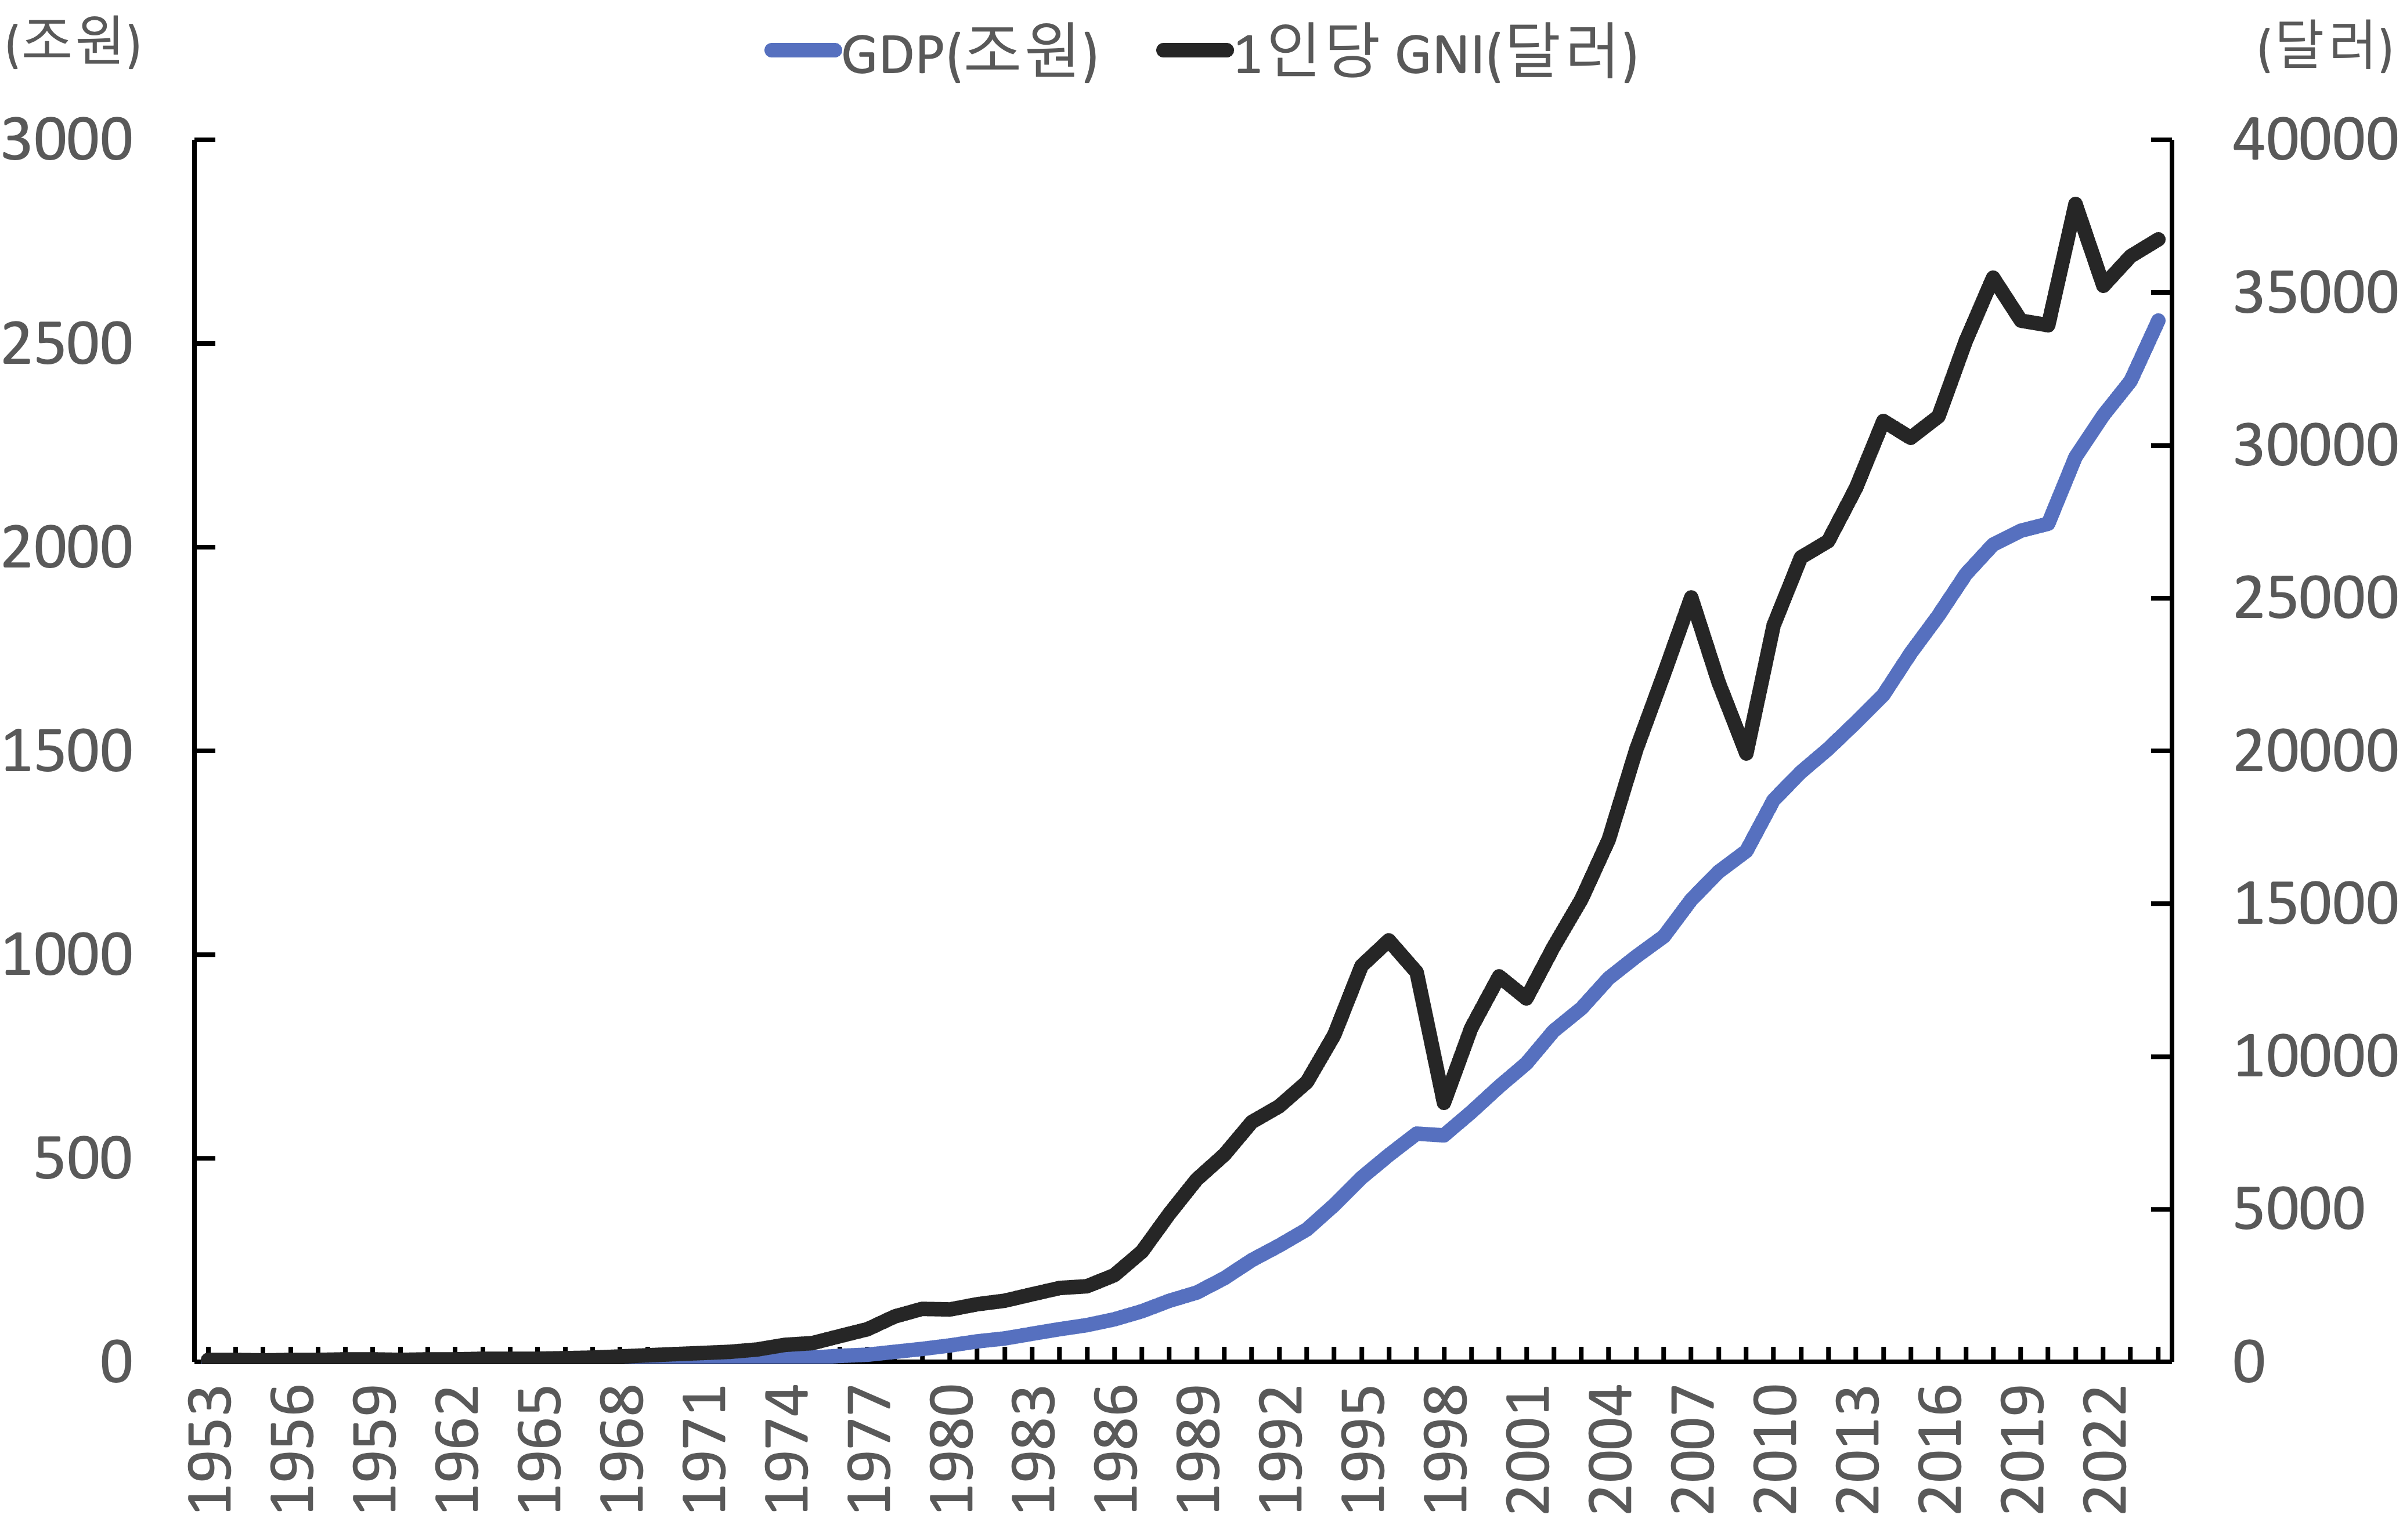
\includegraphics[width=.55\textwidth]{pic/fig_econ_01.png}
    \end{figure}
    \begin{itemize}
        \item 효용을 극대화 하는 분배가 정당한 분배이다.
    \end{itemize}
\end{frame}

\begin{frame}[<+->]
\frametitle{경제성장률}
    \begin{figure}
        \centering
        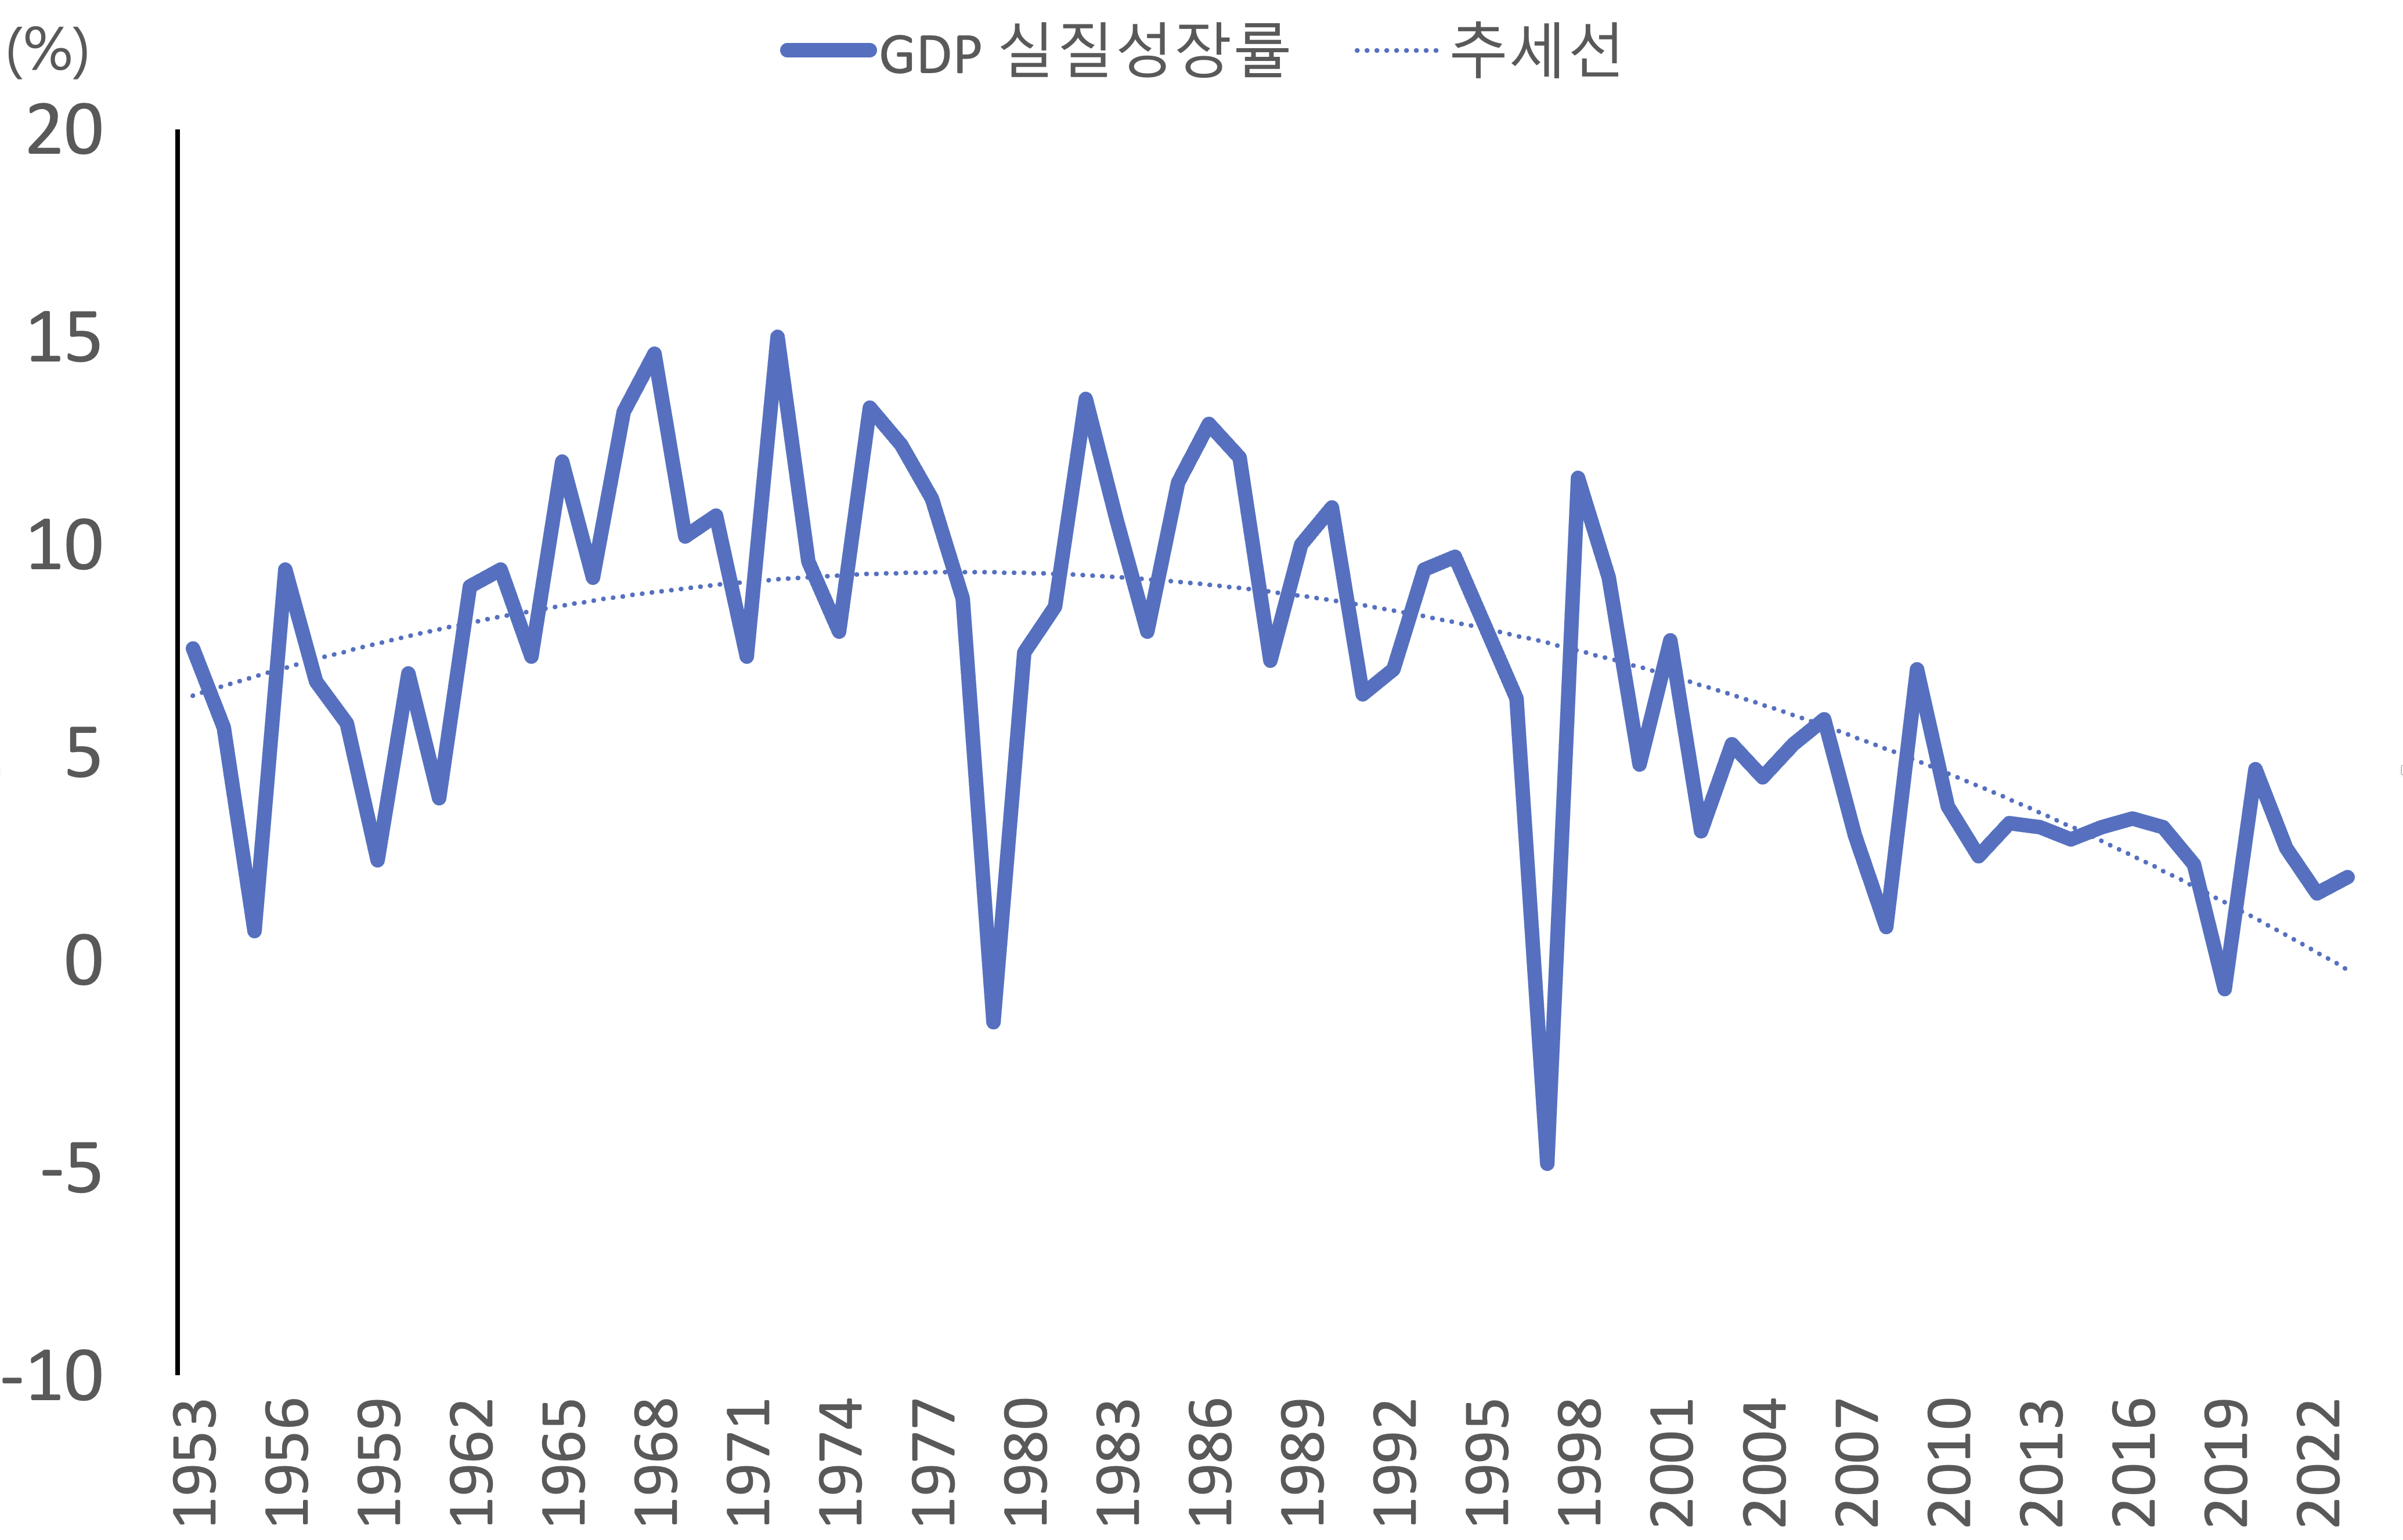
\includegraphics[width=.55\textwidth]{pic/fig_econ_02.png}
    \end{figure}
    \begin{itemize}
        \item 효용을 극대화 하는 분배가 정당한 분배이다. 효용을 극대화 하는 분배가 정당한 분배이다.
    \end{itemize}
\end{frame}

\subsection{산업구조}
\begin{frame}
\frametitle{산업규모\textperiodcentered구조}
\begin{columns}
    \begin{column}{.5\textwidth}
        \begin{figure}
            \centering
            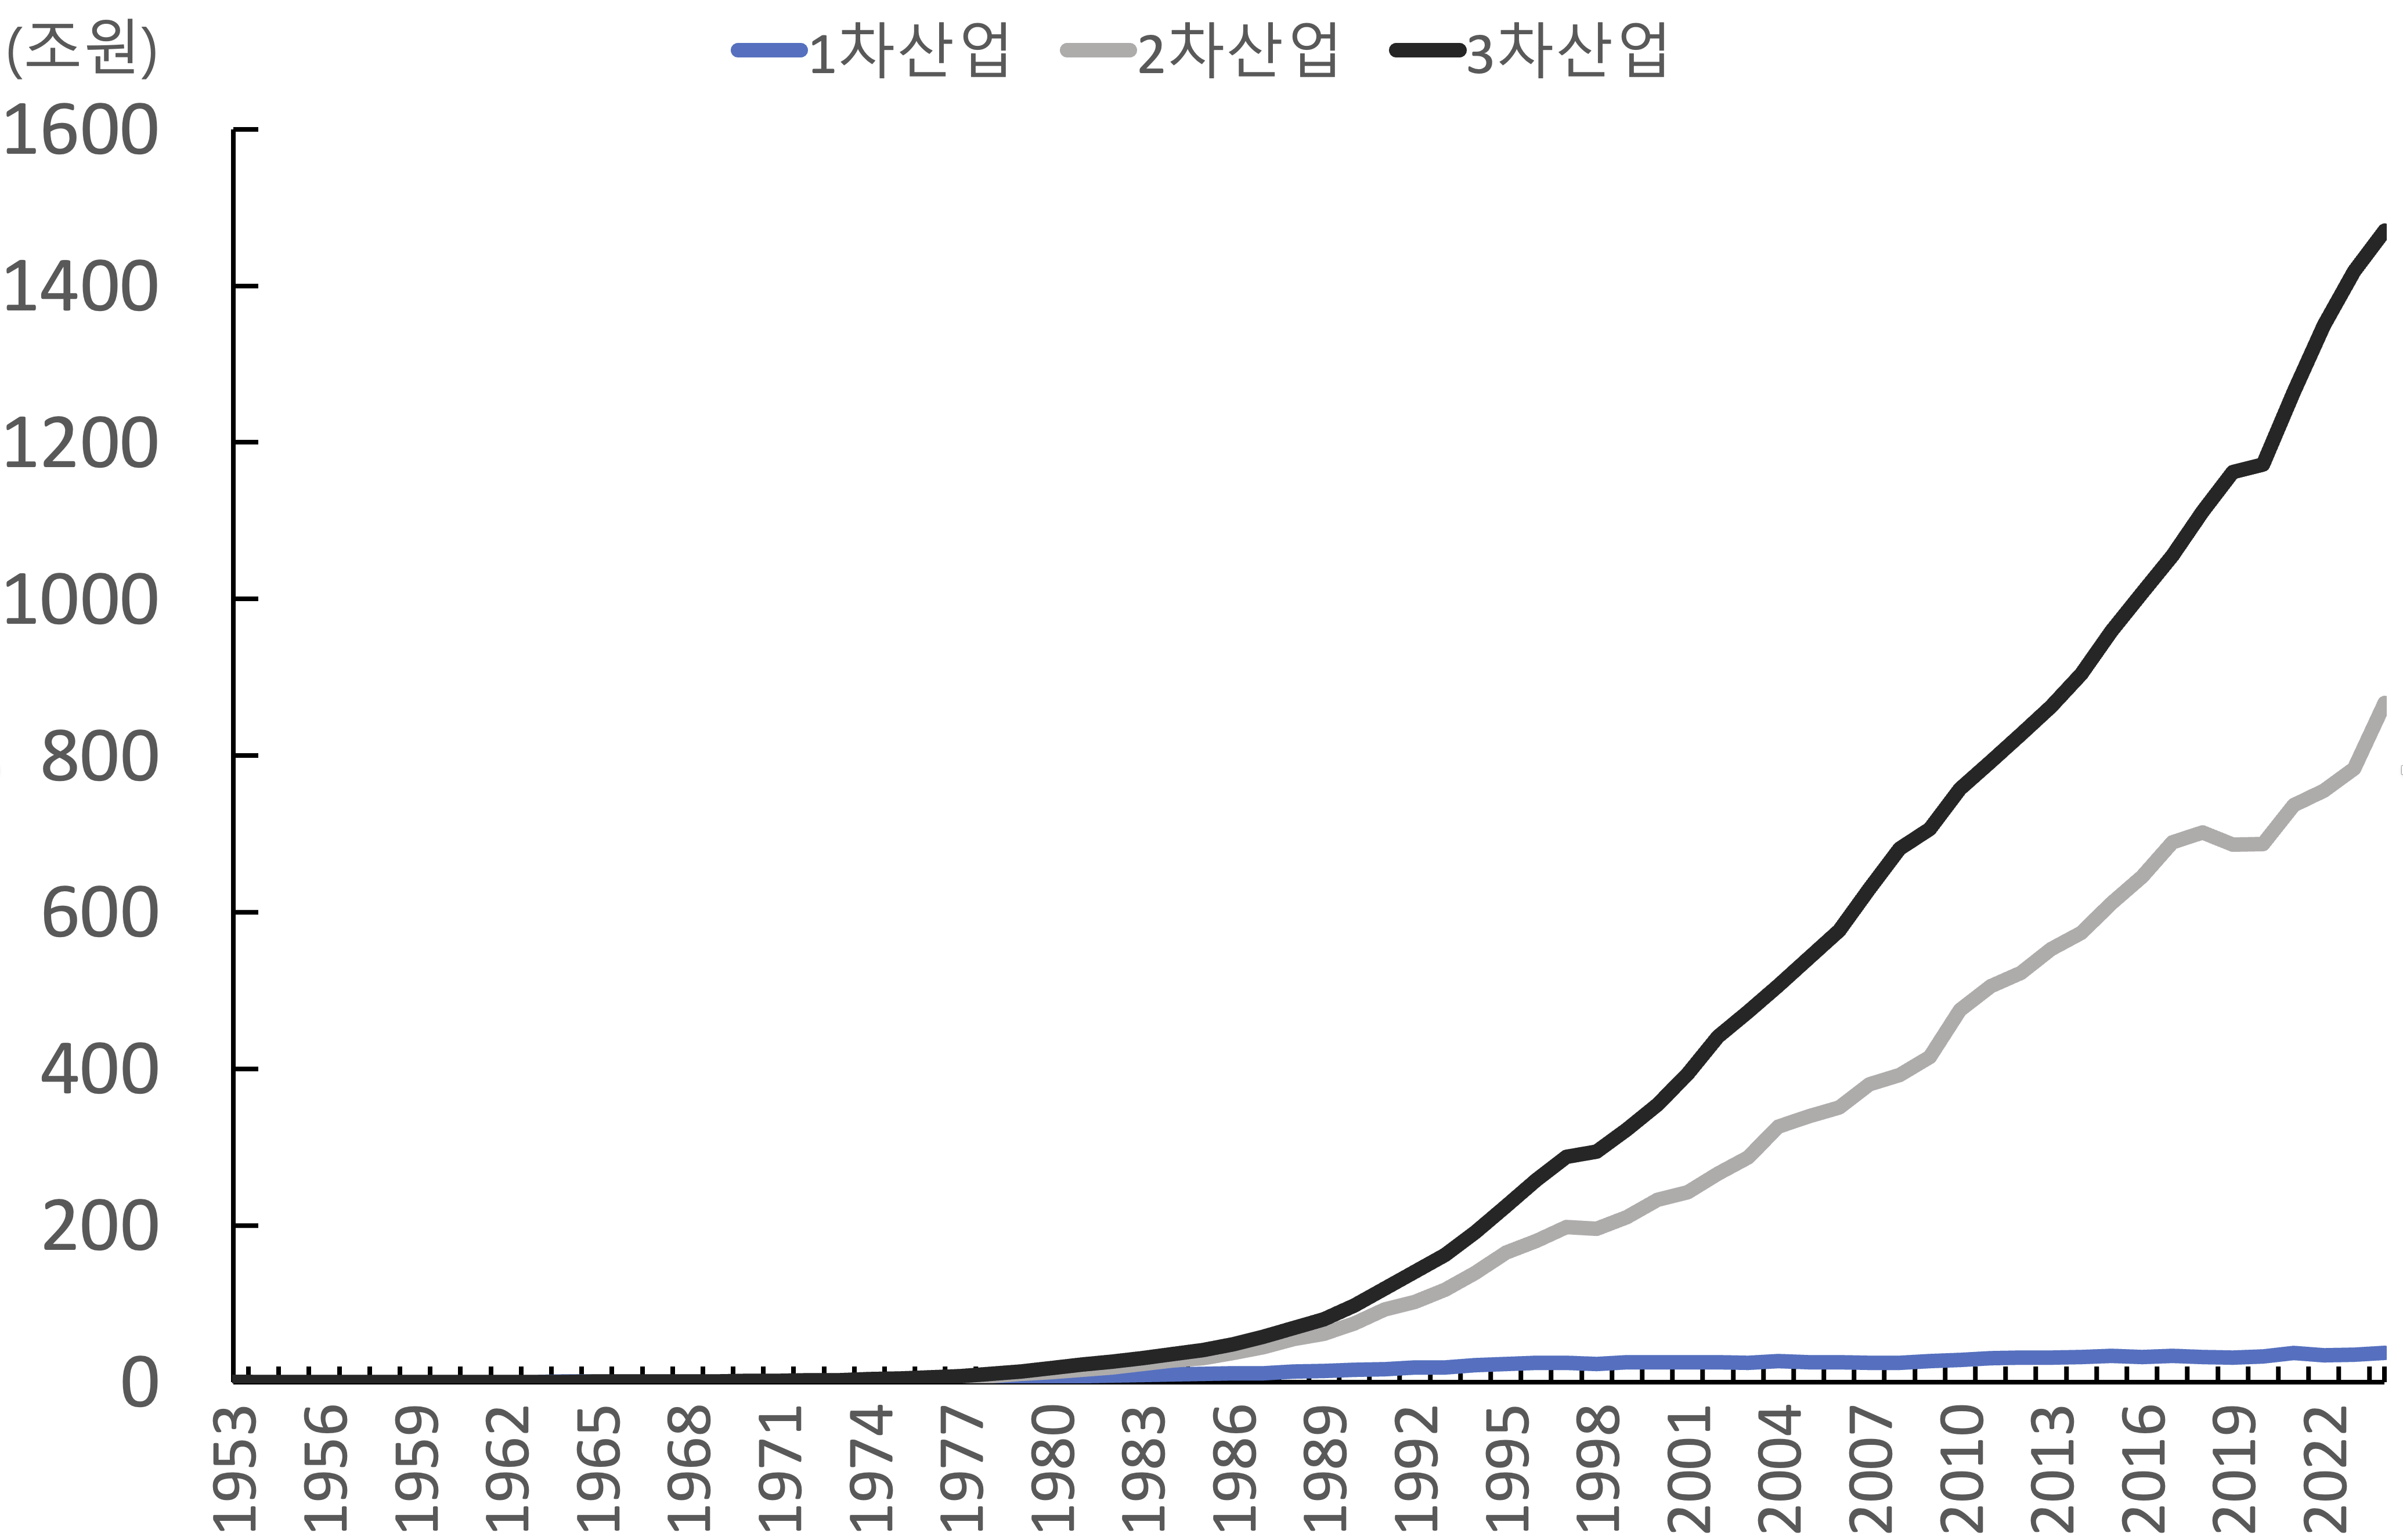
\includegraphics[width=.9\textwidth]{pic/fig_econ_03.png}
        \end{figure}
        \begin{itemize}[<+->]
            \item 효용을 극대화 하는 분배가 정당한 분배이다. 효용을 극대화 하는 분배가 정당한 분배이다.
        \end{itemize}
    \end{column}
    \begin{column}{.5\textwidth}
        \begin{figure}
            \centering
            \only<1|handout:0>{\transparent{0.3}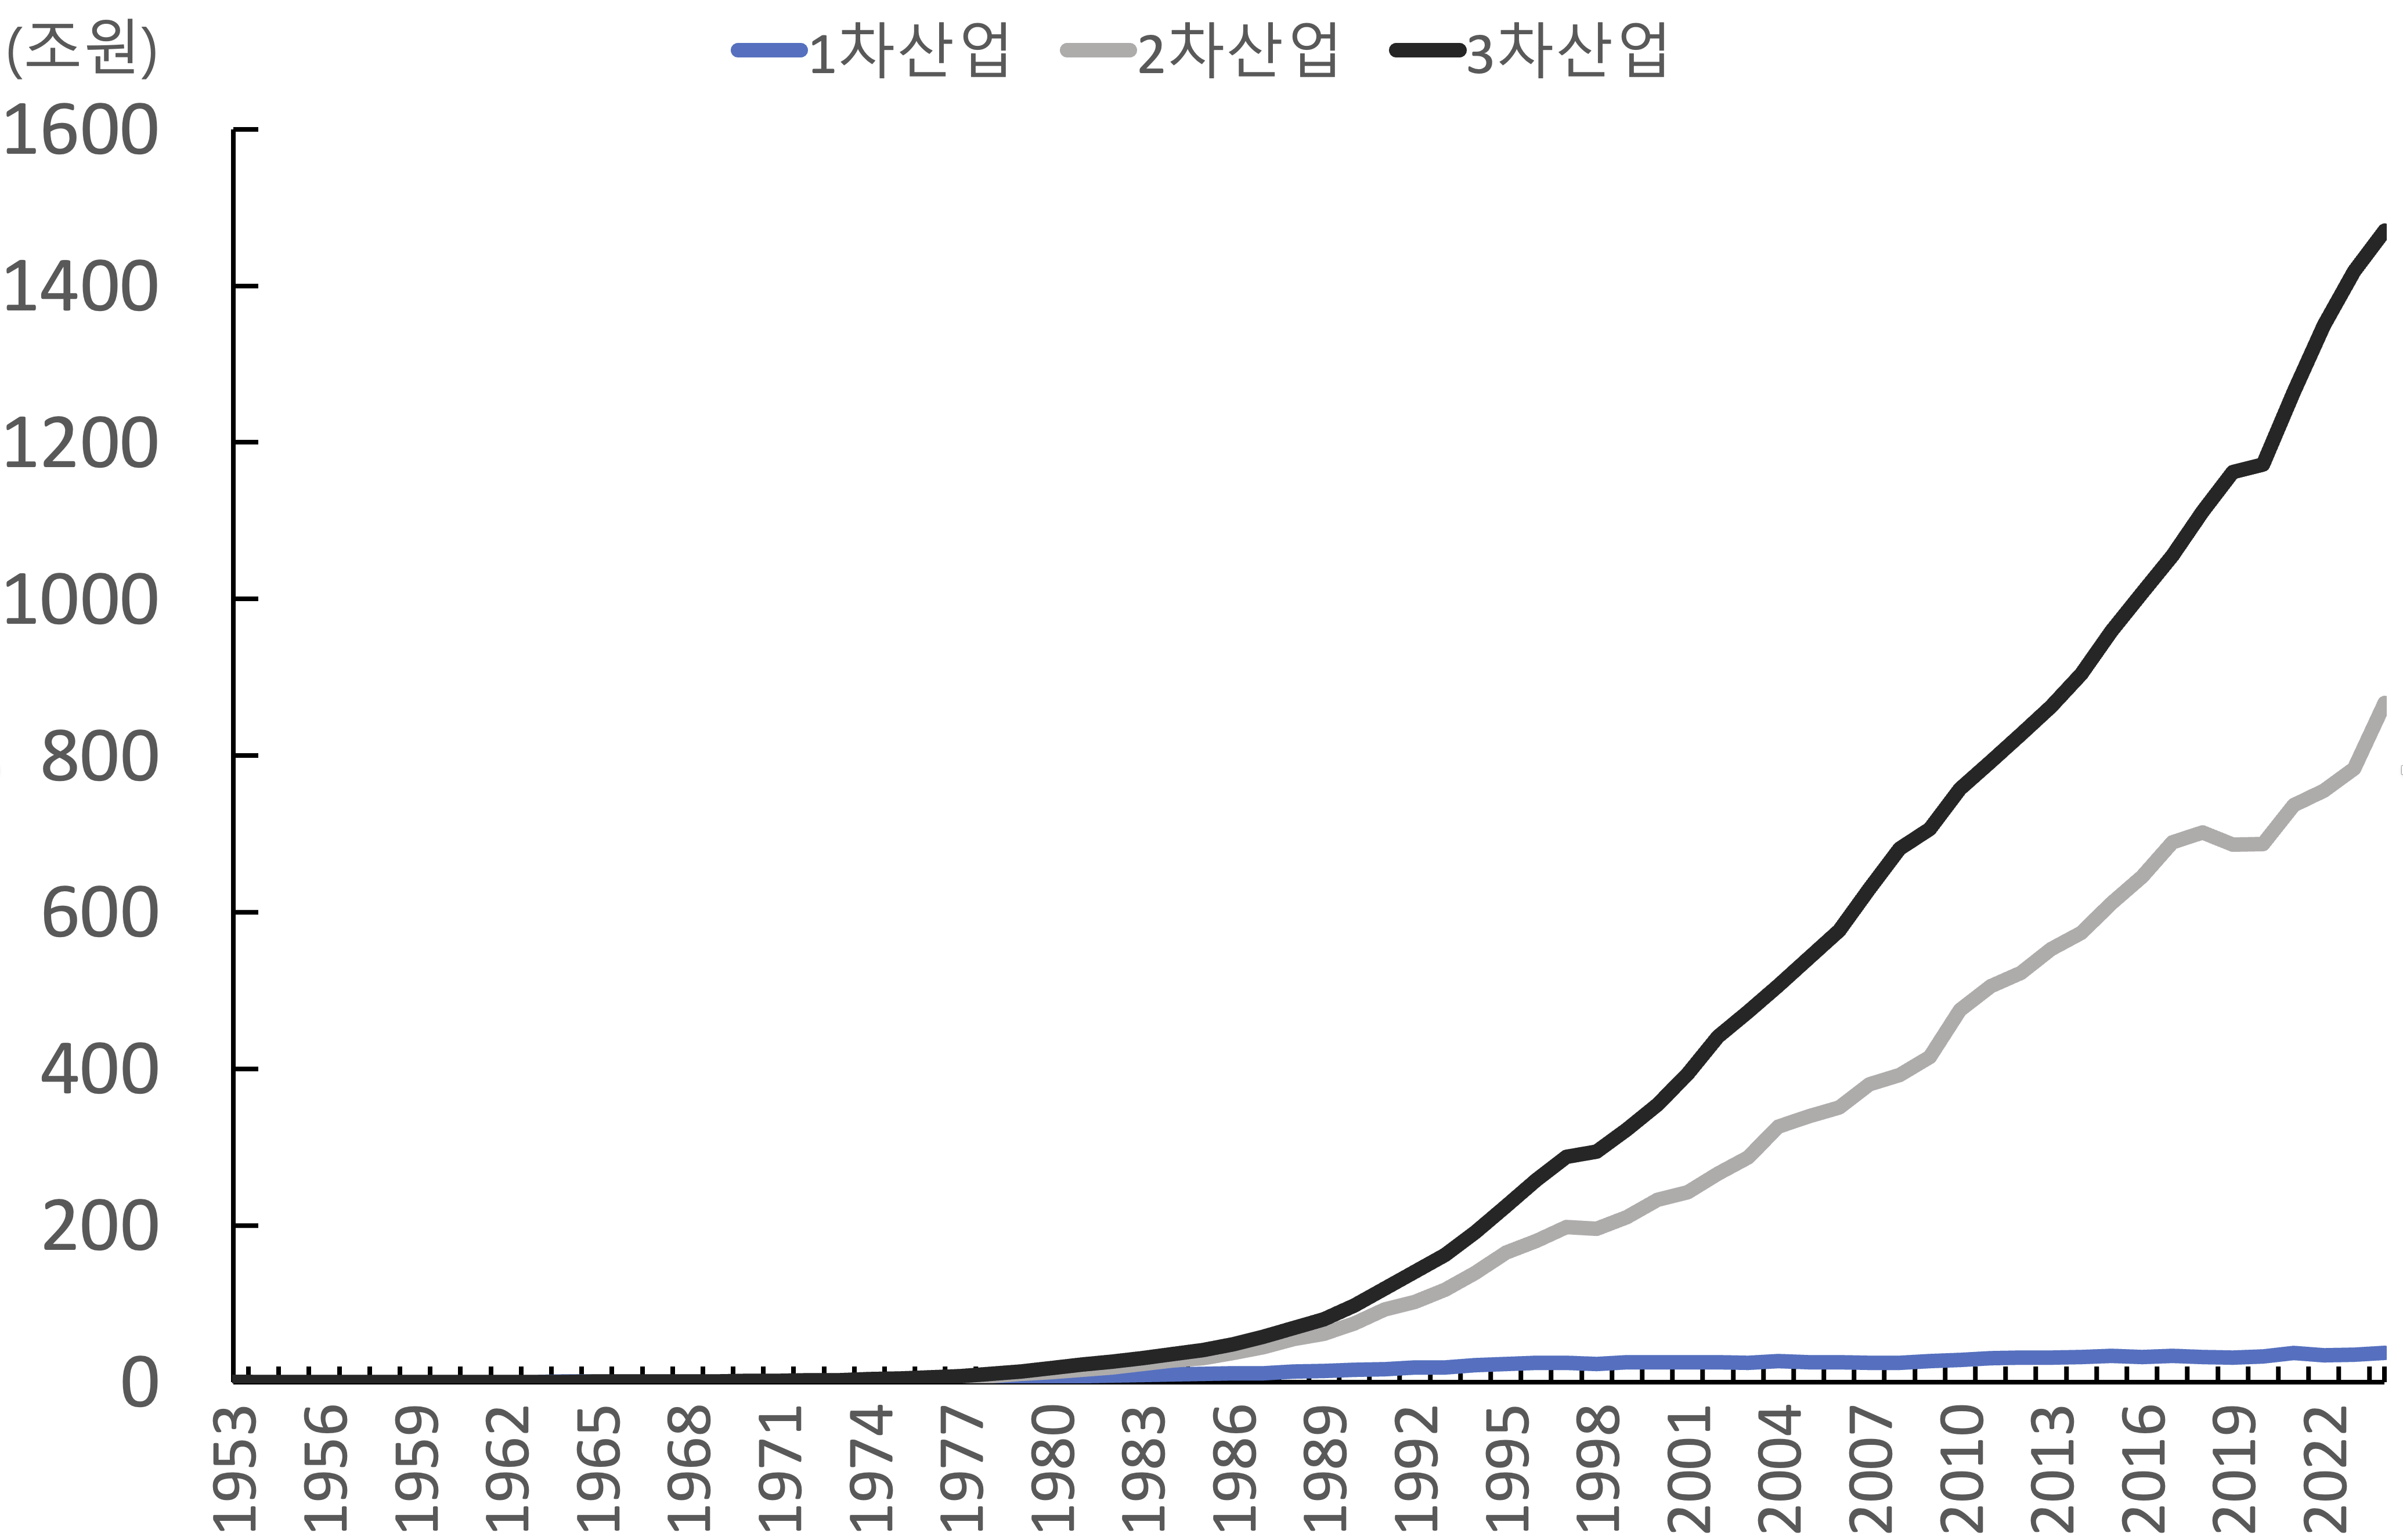
\includegraphics[width=.7\textwidth]{pic/fig_econ_03.png}} % 첫 번째 슬라이드: 투명하게 표시
            \only<2>{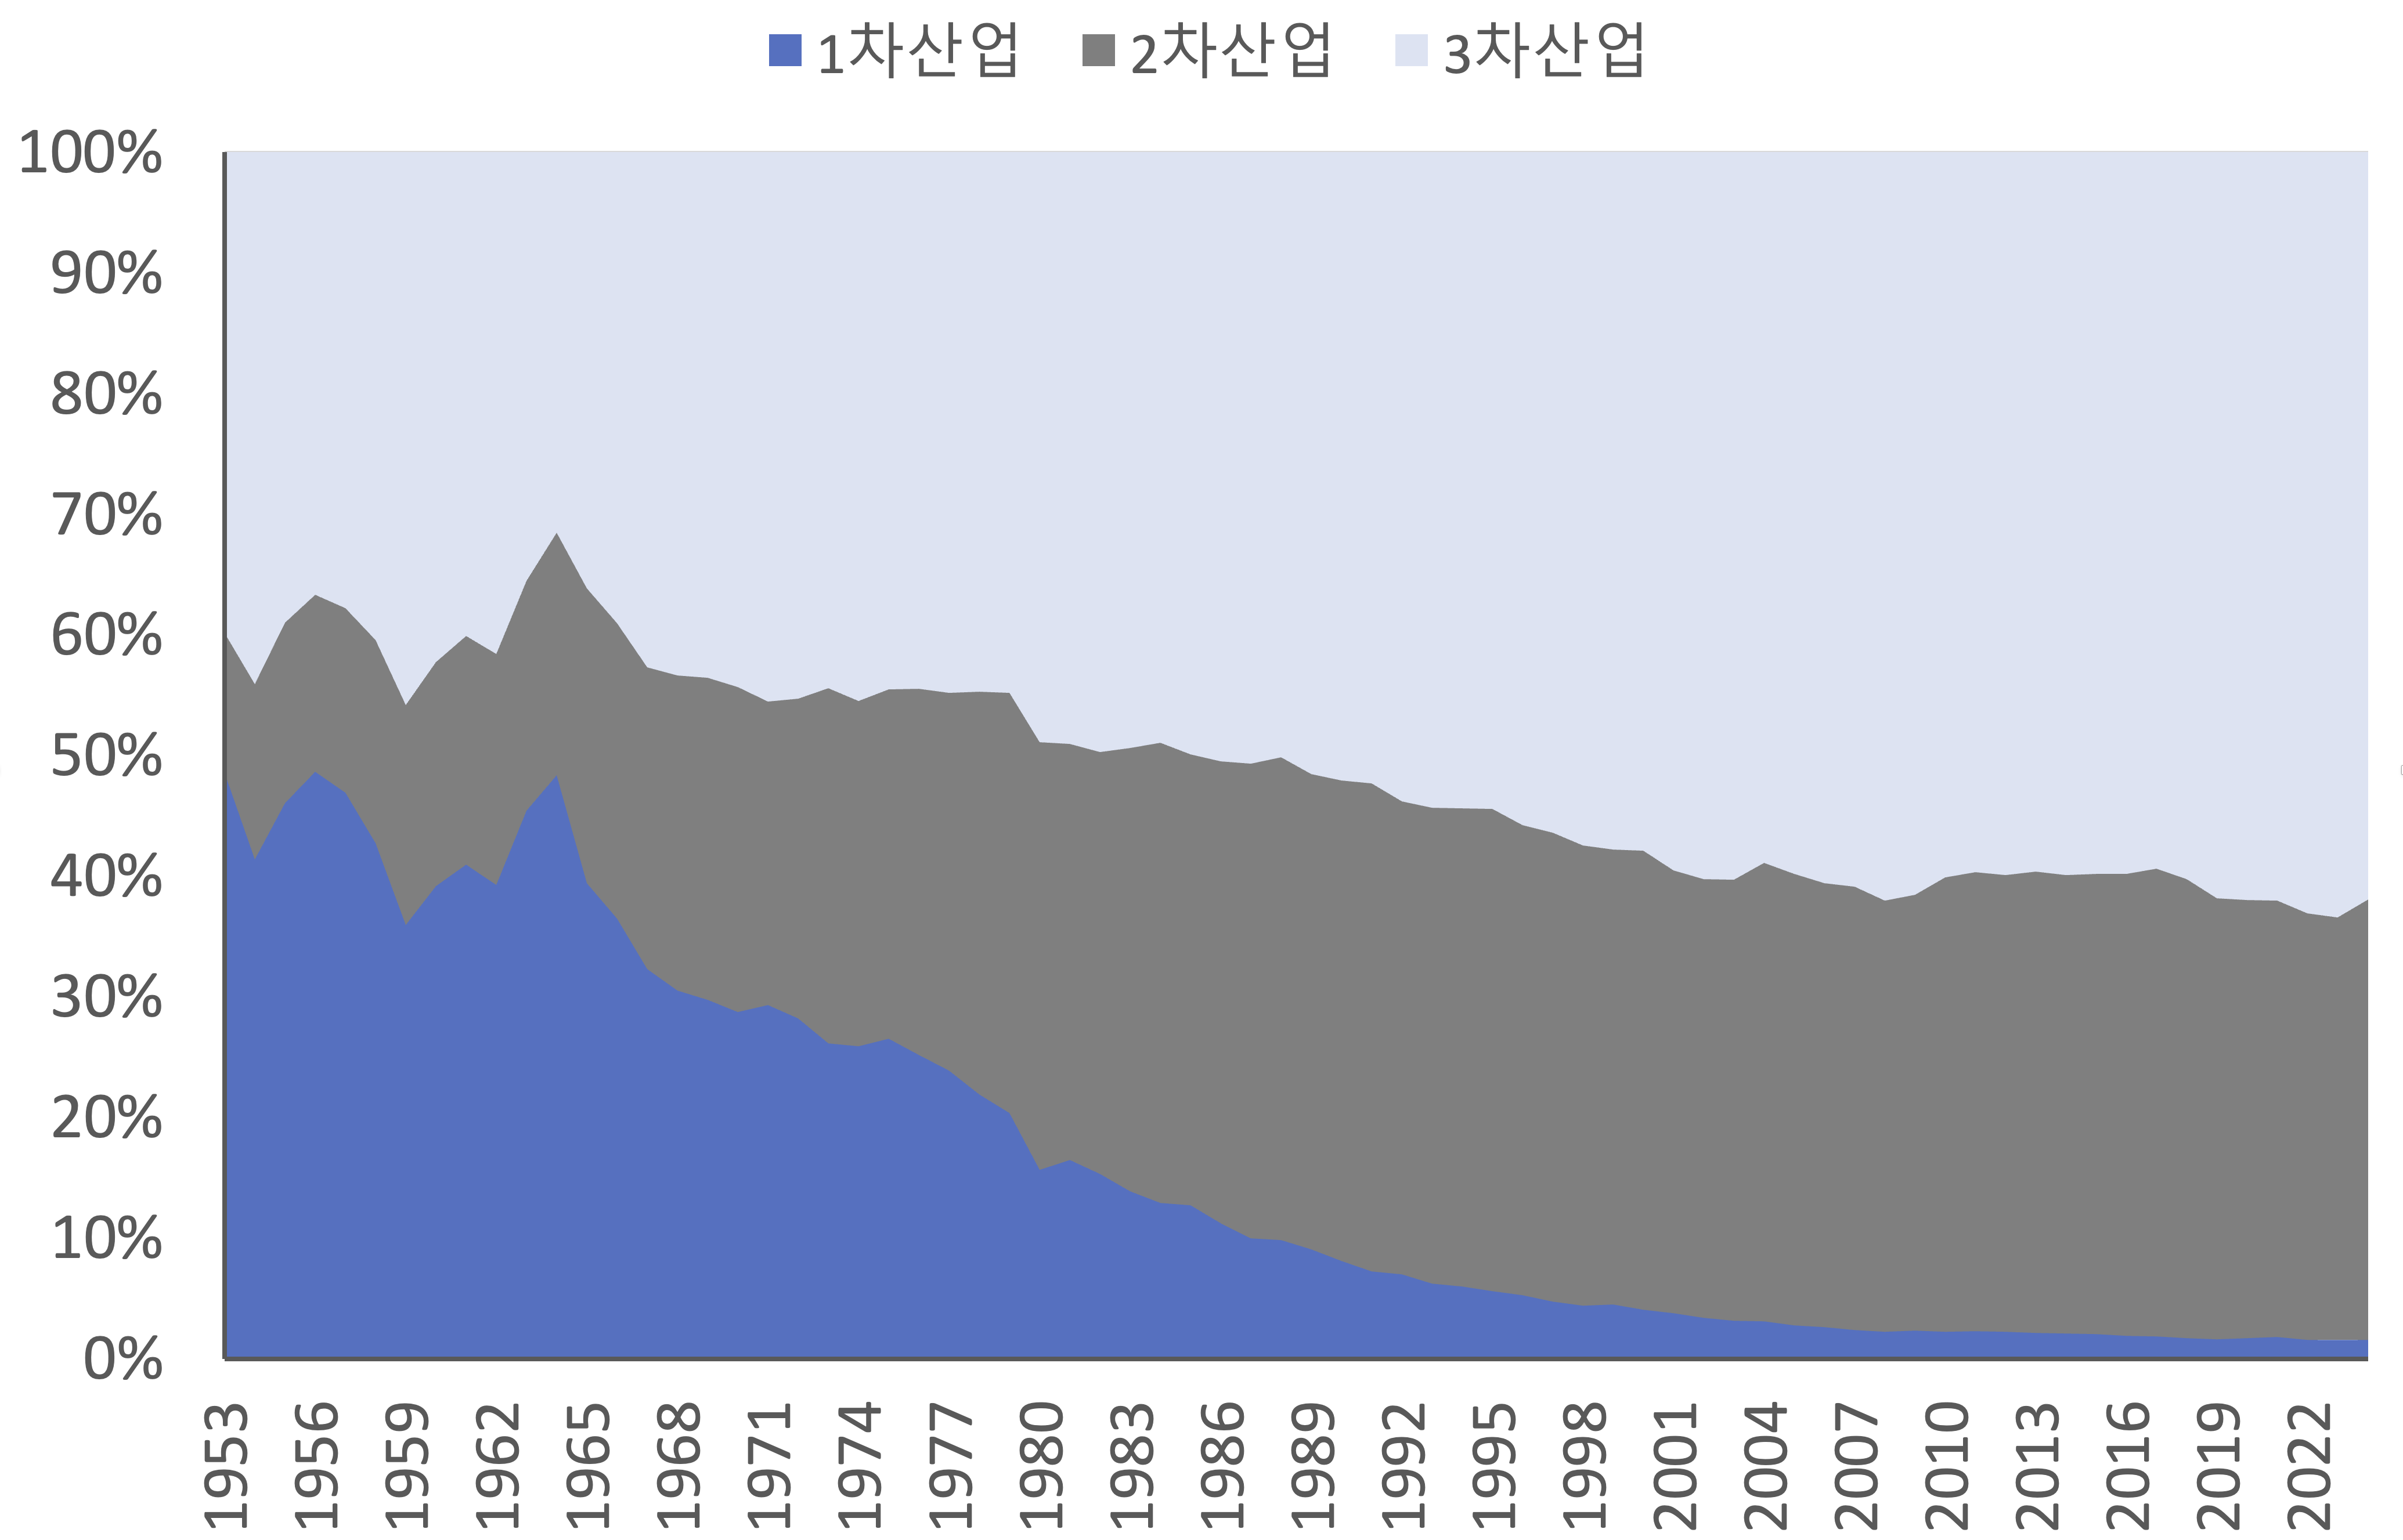
\includegraphics[width=.9\textwidth]{pic/fig_econ_04.png}} % 두 번째 슬라이드: 선명하게 표시
            \\
            \begin{itemize}[<+->]
                \item 효용을 극대화 하는 분배가 정당한 분배이다. 효용을 극대화 하는 분배가 정당한 분배이다.
            \end{itemize}
        \end{figure}
    \end{column}
\end{columns}
\end{frame}

\subsection{무역}
\begin{frame}[<+->]
\frametitle{경제성장}
    \begin{figure}
        \centering
        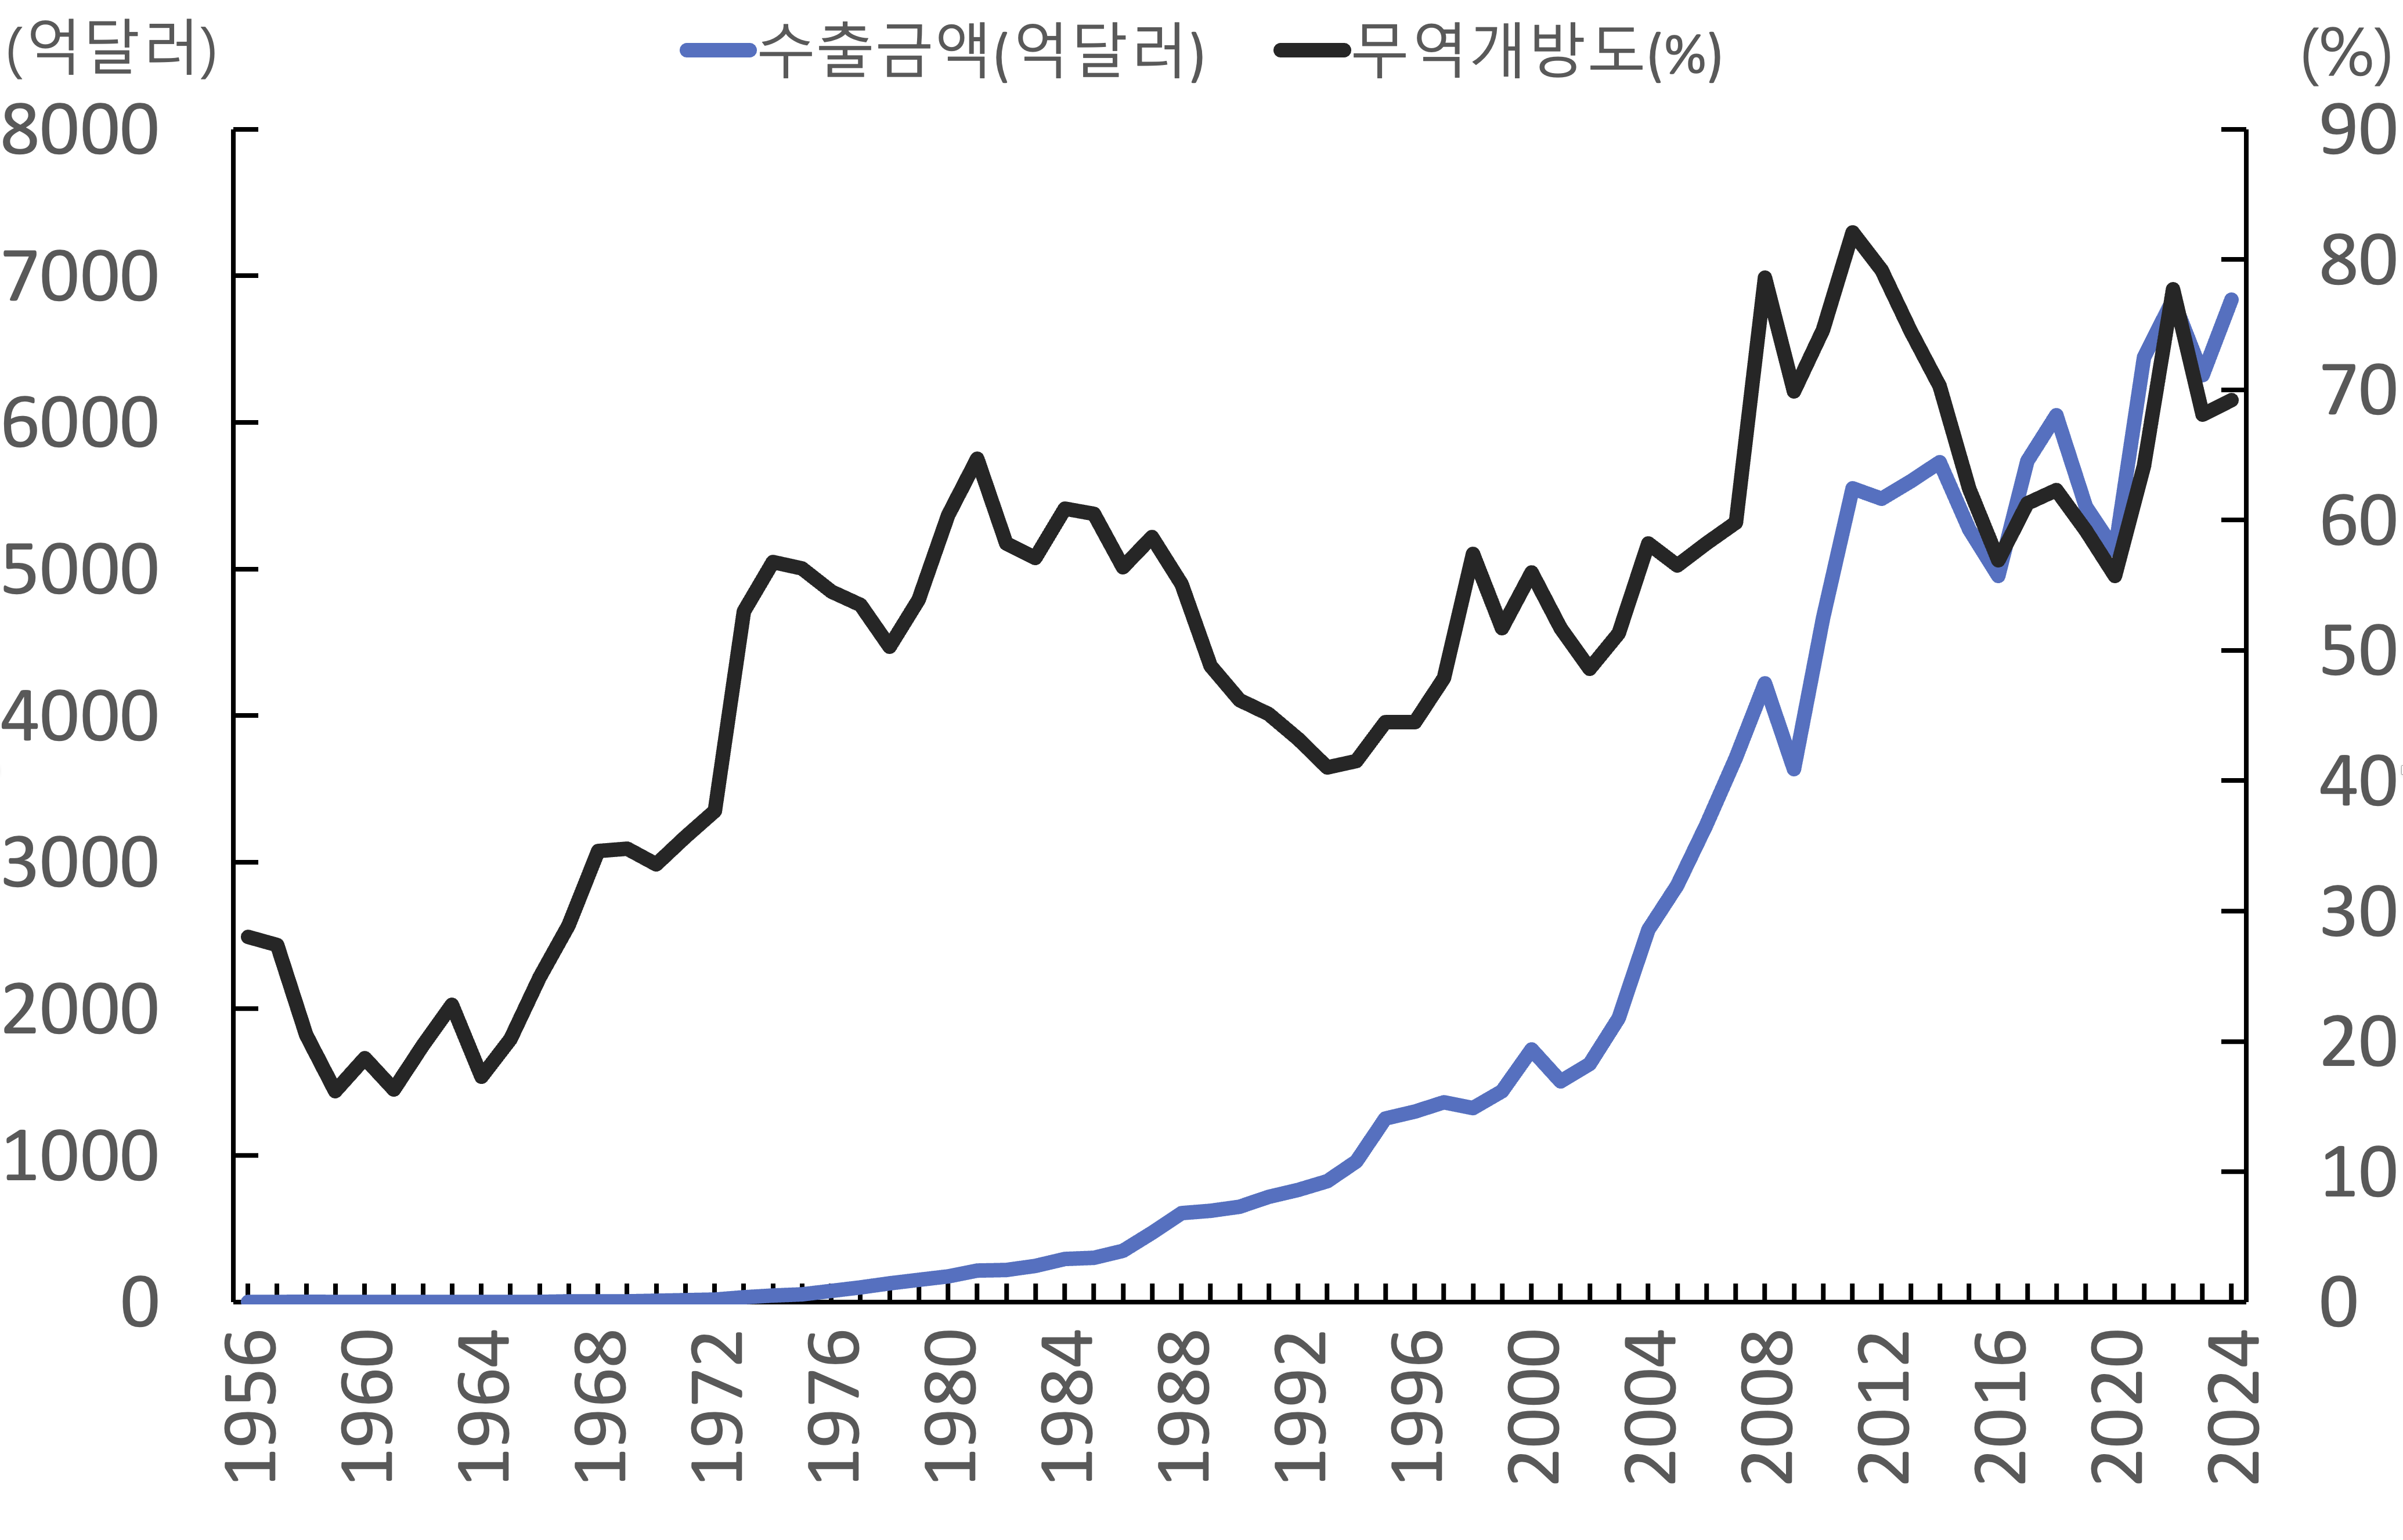
\includegraphics[width=.55\textwidth]{pic/fig_econ_05.png}
    \end{figure}
    \begin{itemize}
        \item 효용을 극대화 하는 분배가 정당한 분배이다.
    \end{itemize}
\end{frame}

\subsection{외환}
\begin{frame}[<+->]
\frametitle{경제성장}
    \begin{figure}
        \centering
        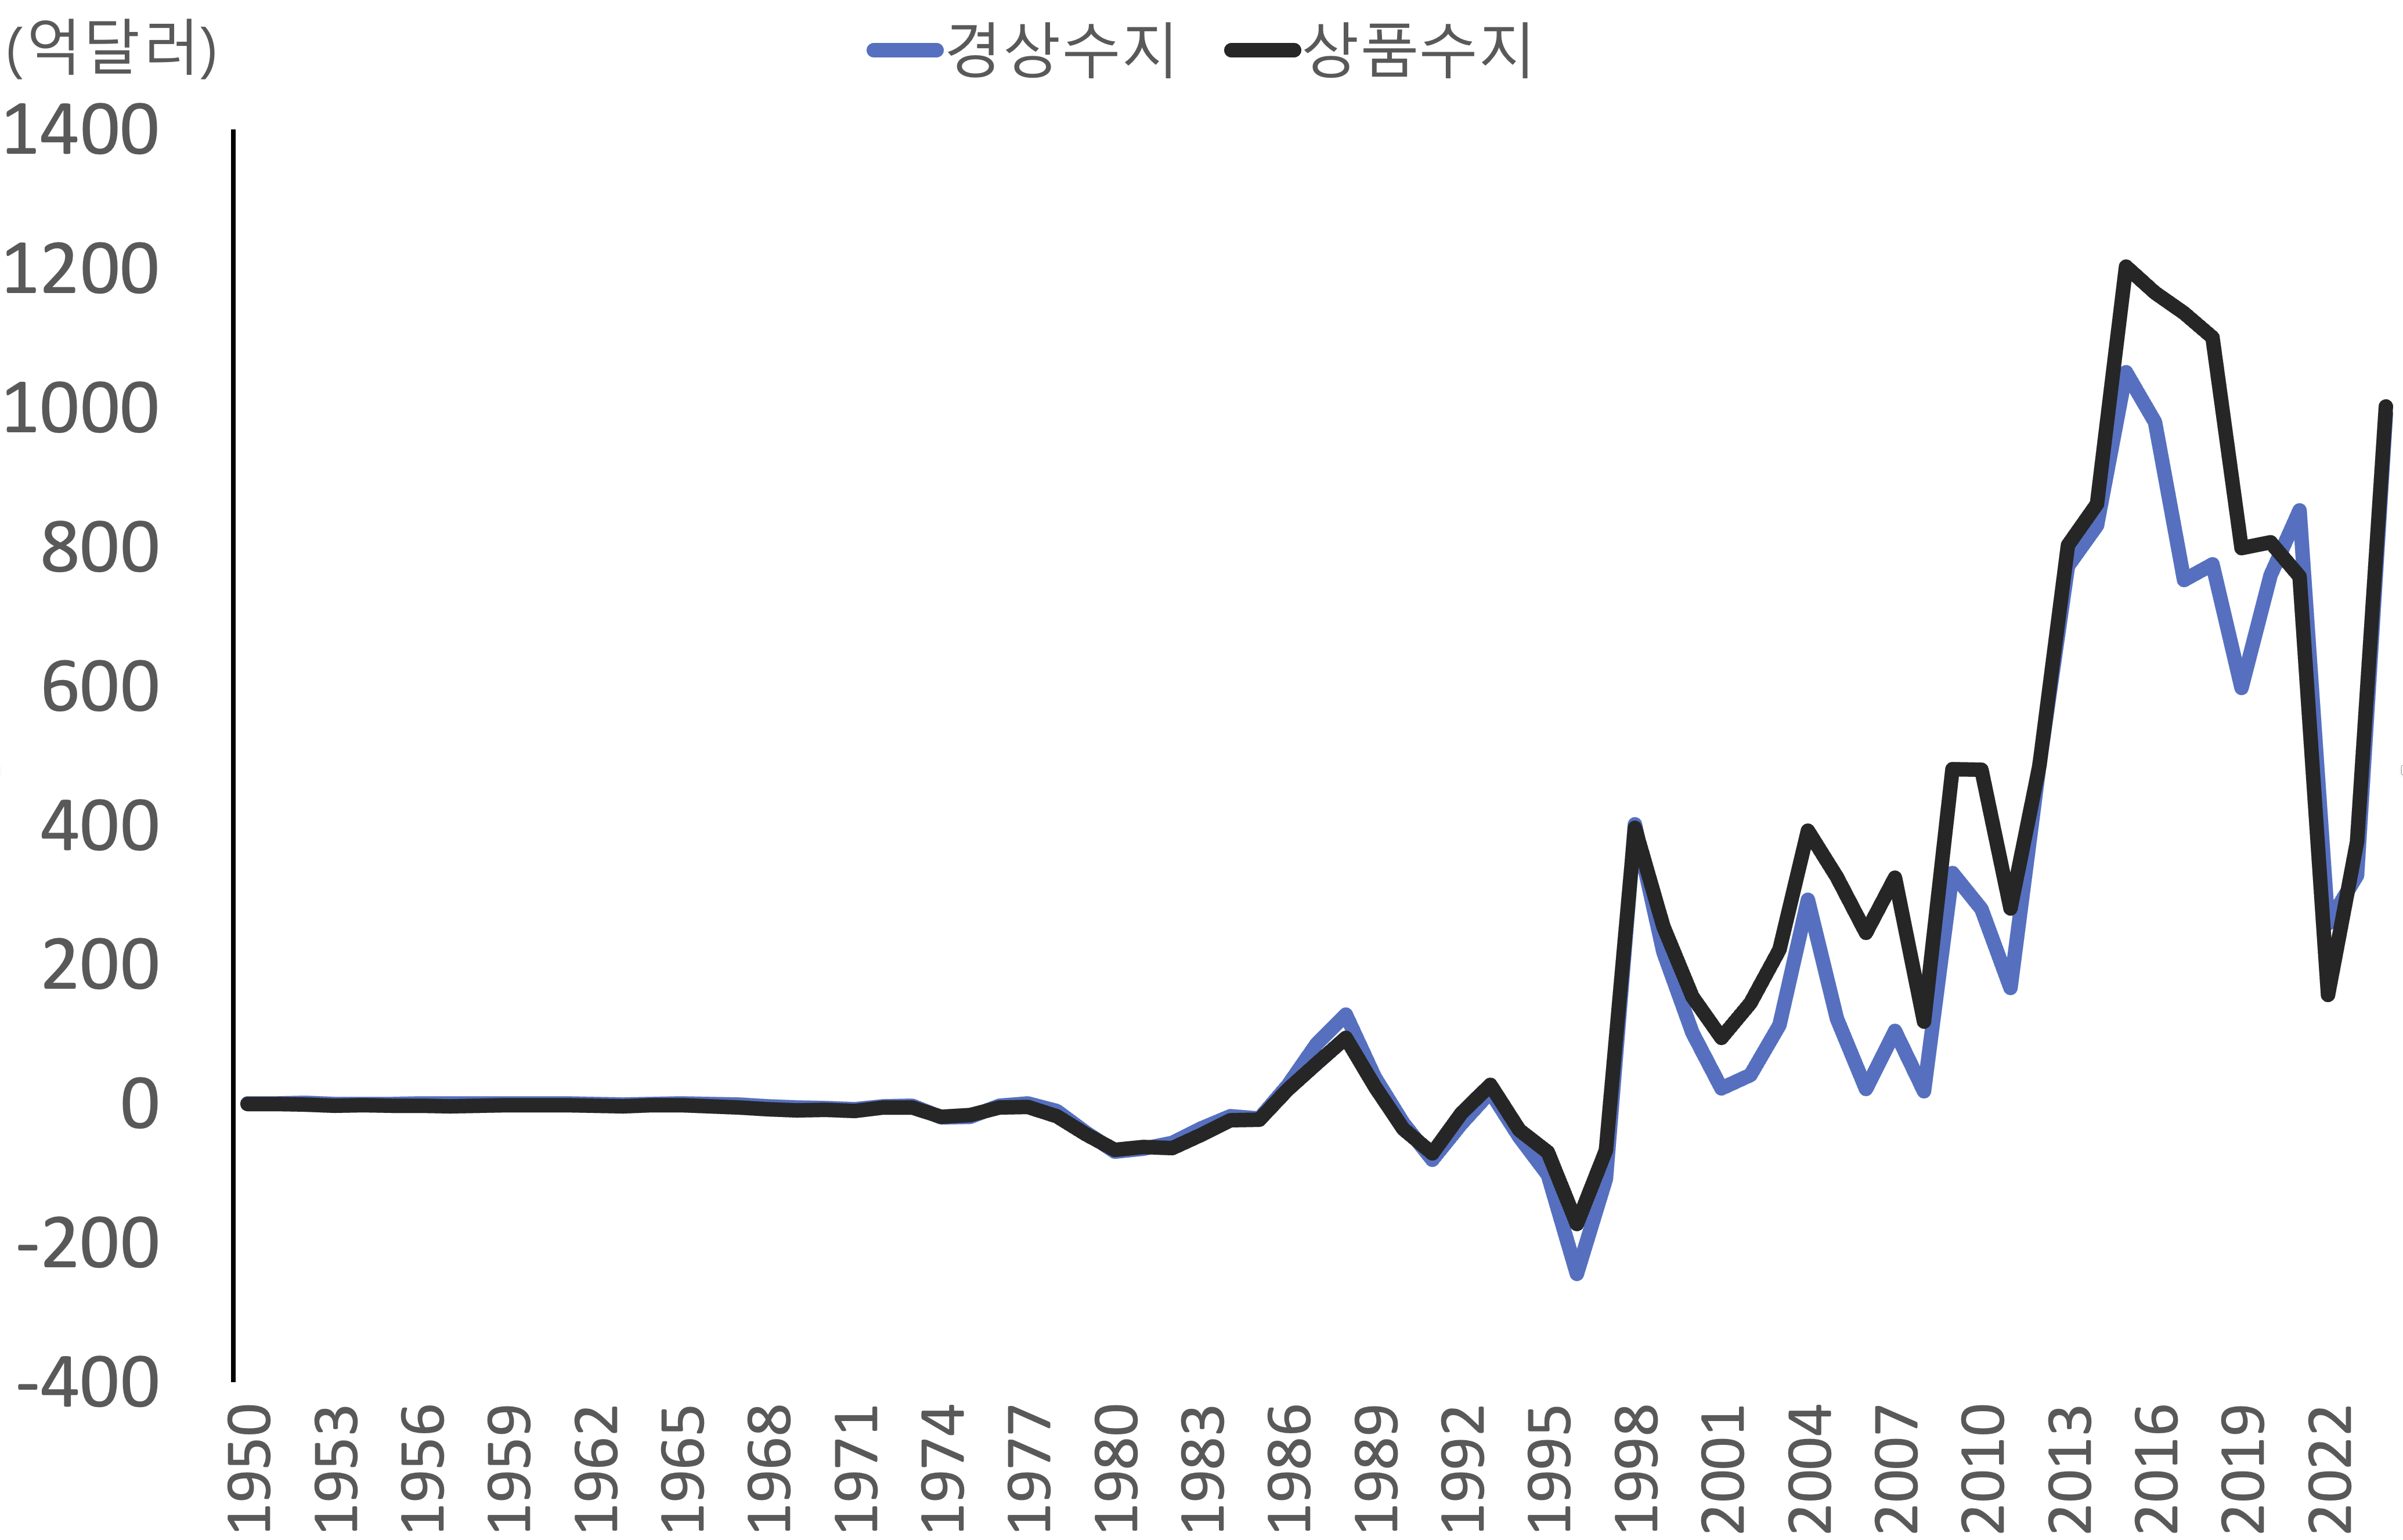
\includegraphics[width=.55\textwidth]{pic/fig_econ_06.png}
    \end{figure}
    \begin{itemize}
        \item 효용을 극대화 하는 분배가 정당한 분배이다.
    \end{itemize}
\end{frame}

\subsection{정부지출}
\begin{frame}[<+->]
\frametitle{경제성장}
    \begin{figure}
        \centering
        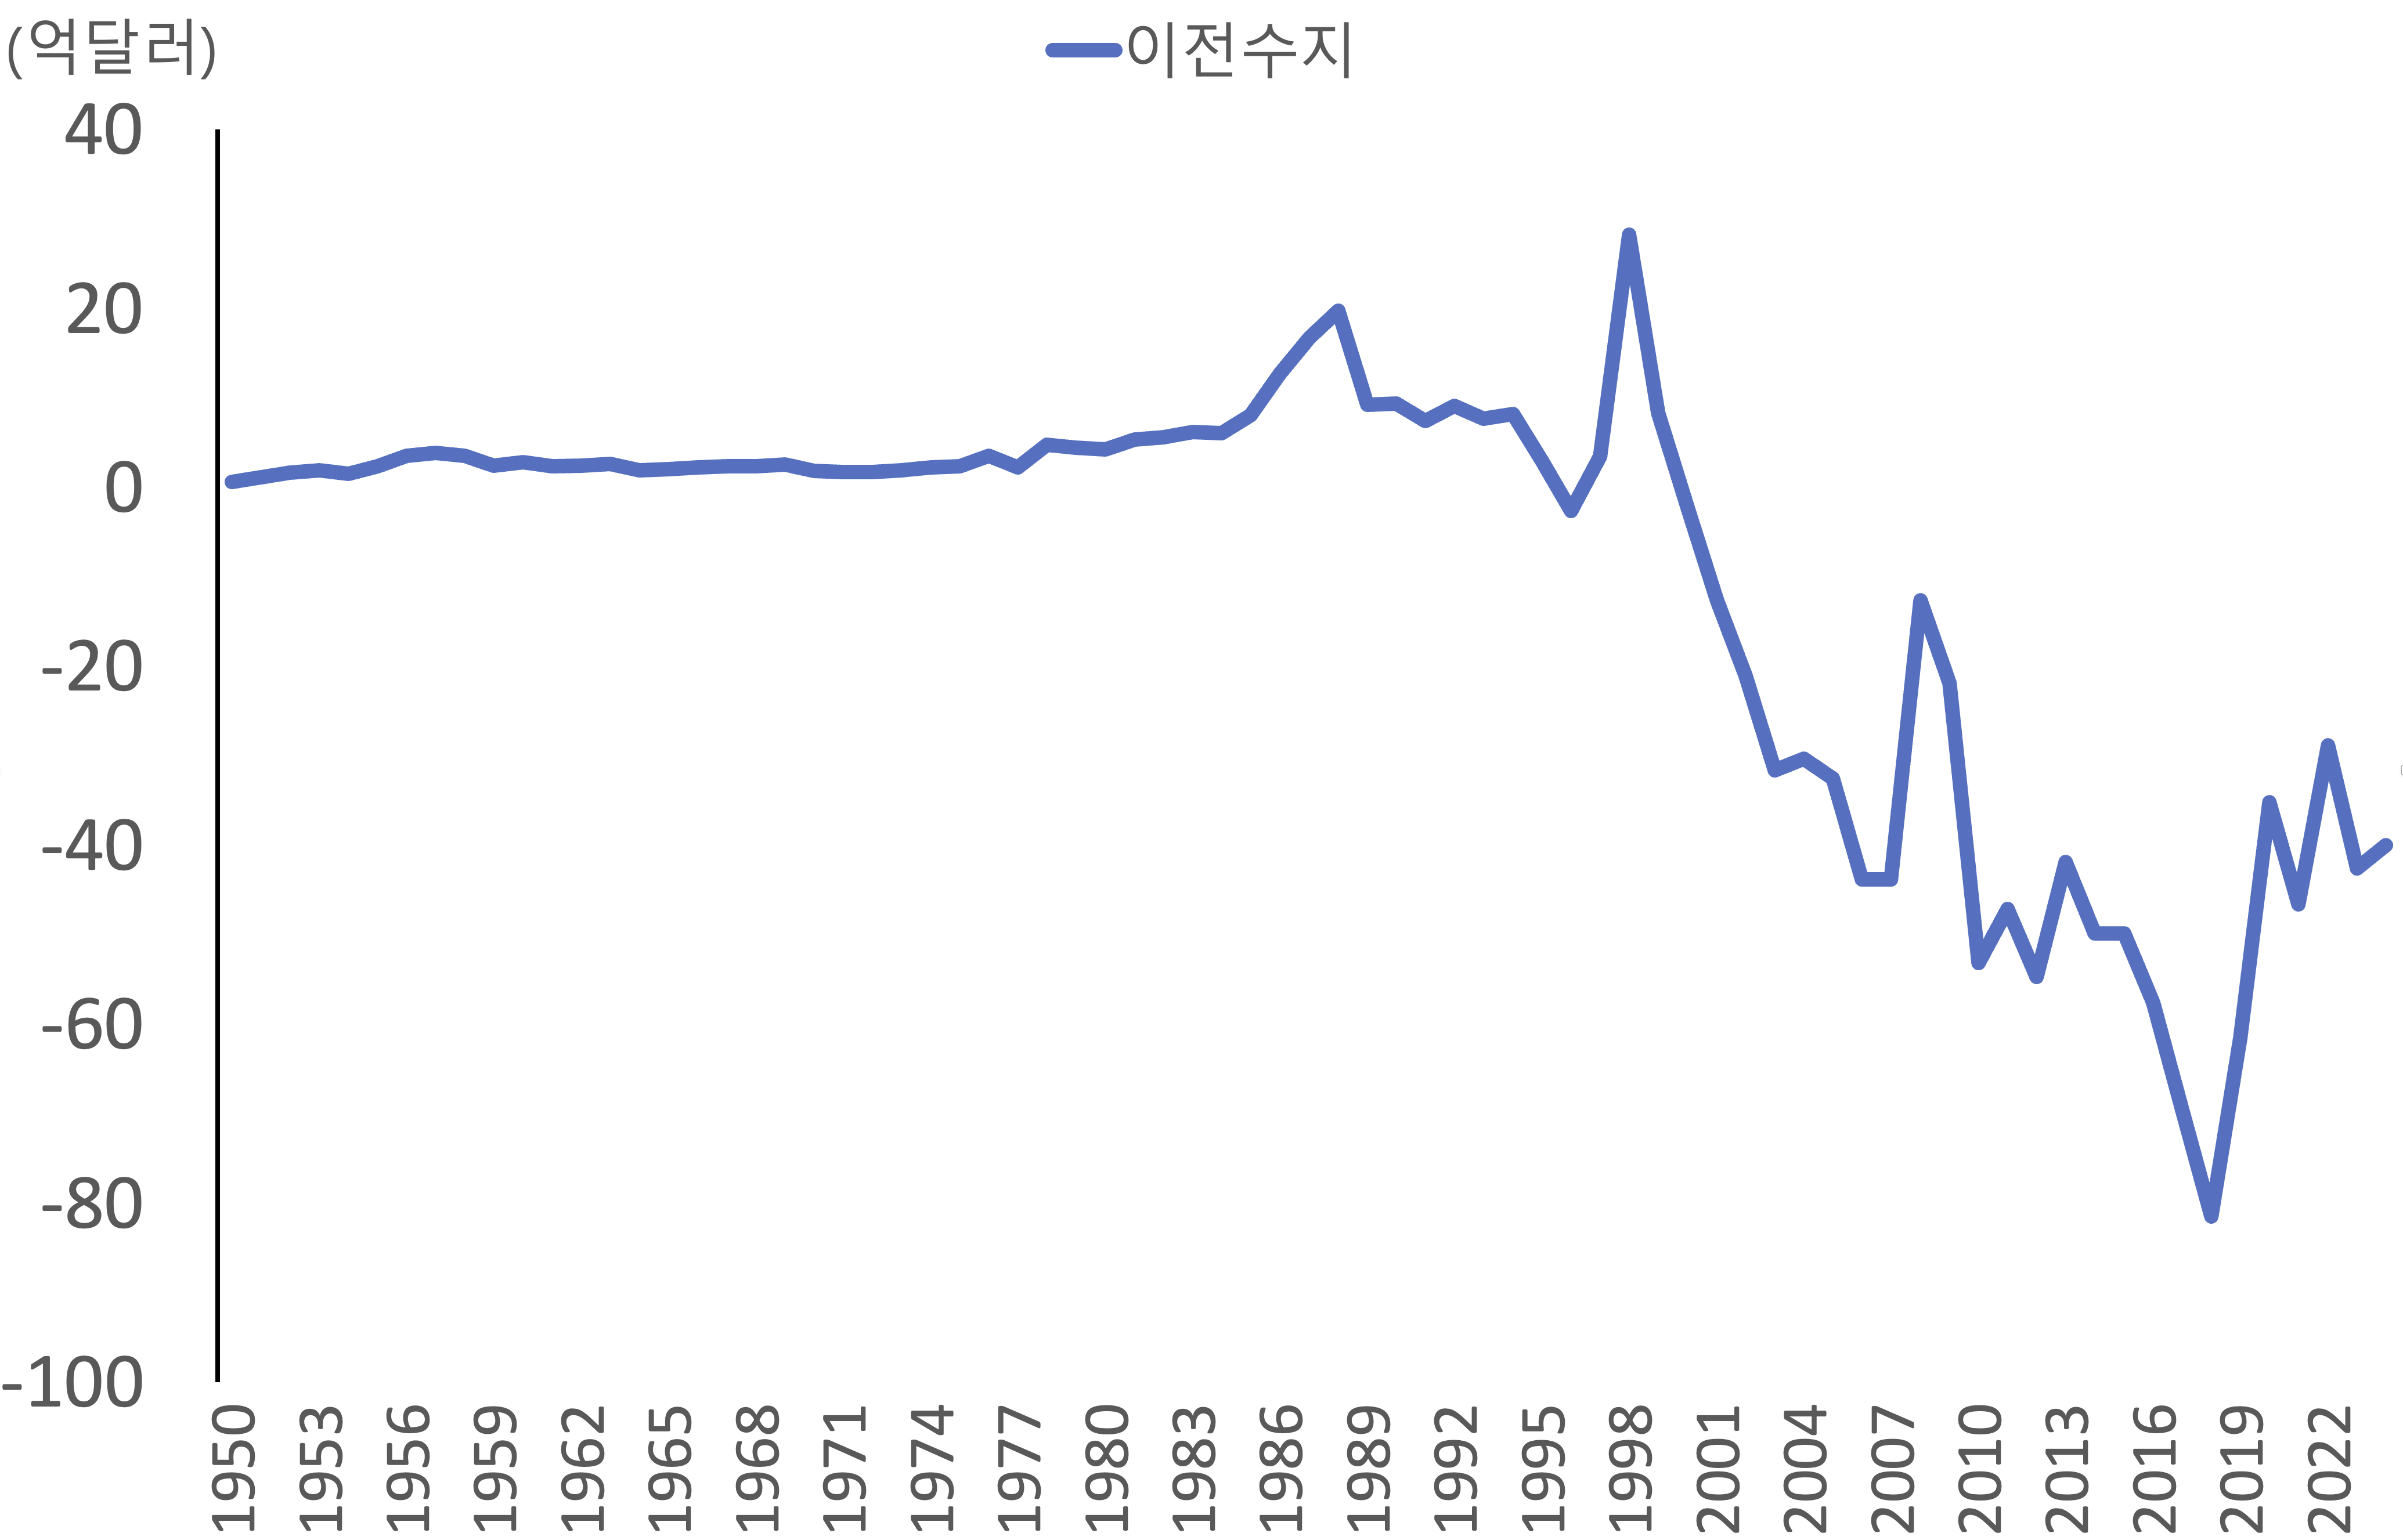
\includegraphics[width=.55\textwidth]{pic/fig_econ_07.png}
    \end{figure}
    \begin{itemize}
        \item 효용을 극대화 하는 분배가 정당한 분배이다.
    \end{itemize}
\end{frame}

\section{소득•소비•자산 분야}%
\subsection{소득}
\begin{frame}[<+->]
\frametitle{가구소득}
    \begin{figure}
        \centering
        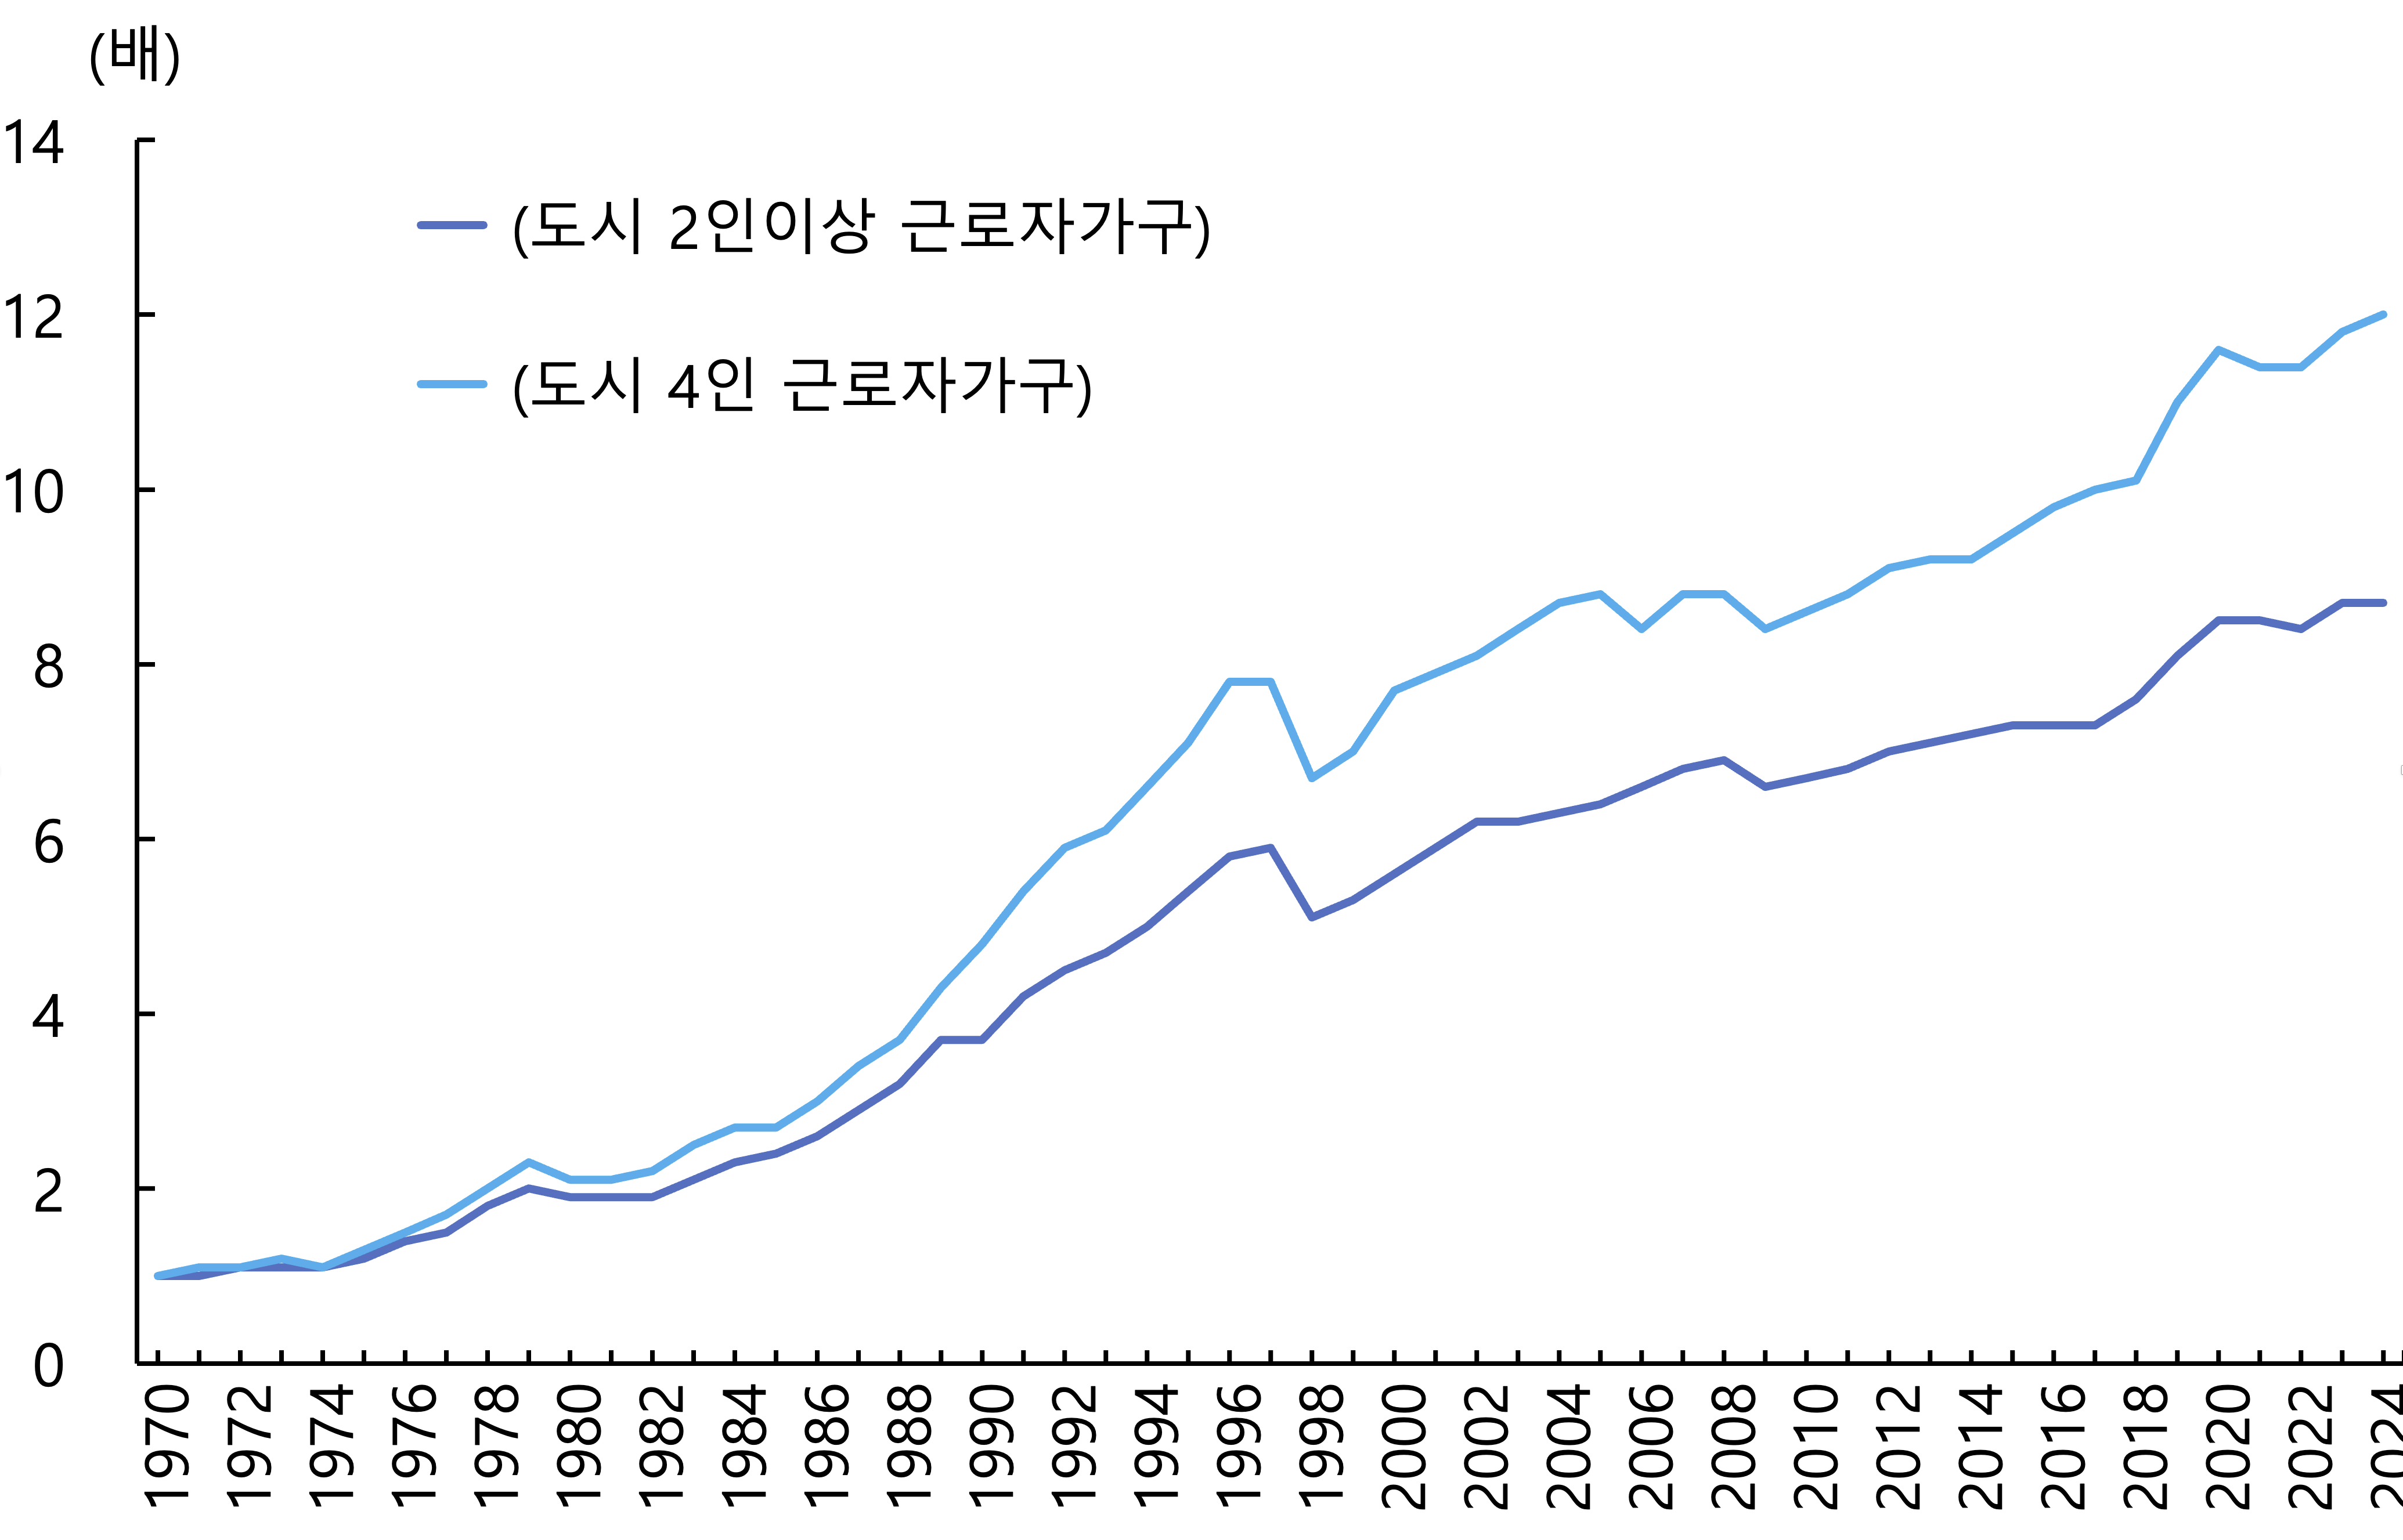
\includegraphics[width=.55\textwidth]{pic/fig_ineq_01.png}
    \end{figure}
    \begin{itemize}
        \item 효용을 극대화 하는 분배가 정당한 분배이다.
    \end{itemize}
\end{frame}

\subsection{물가}
\begin{frame}[<+->]
\frametitle{소비자물가}
    \begin{figure}
        \centering
        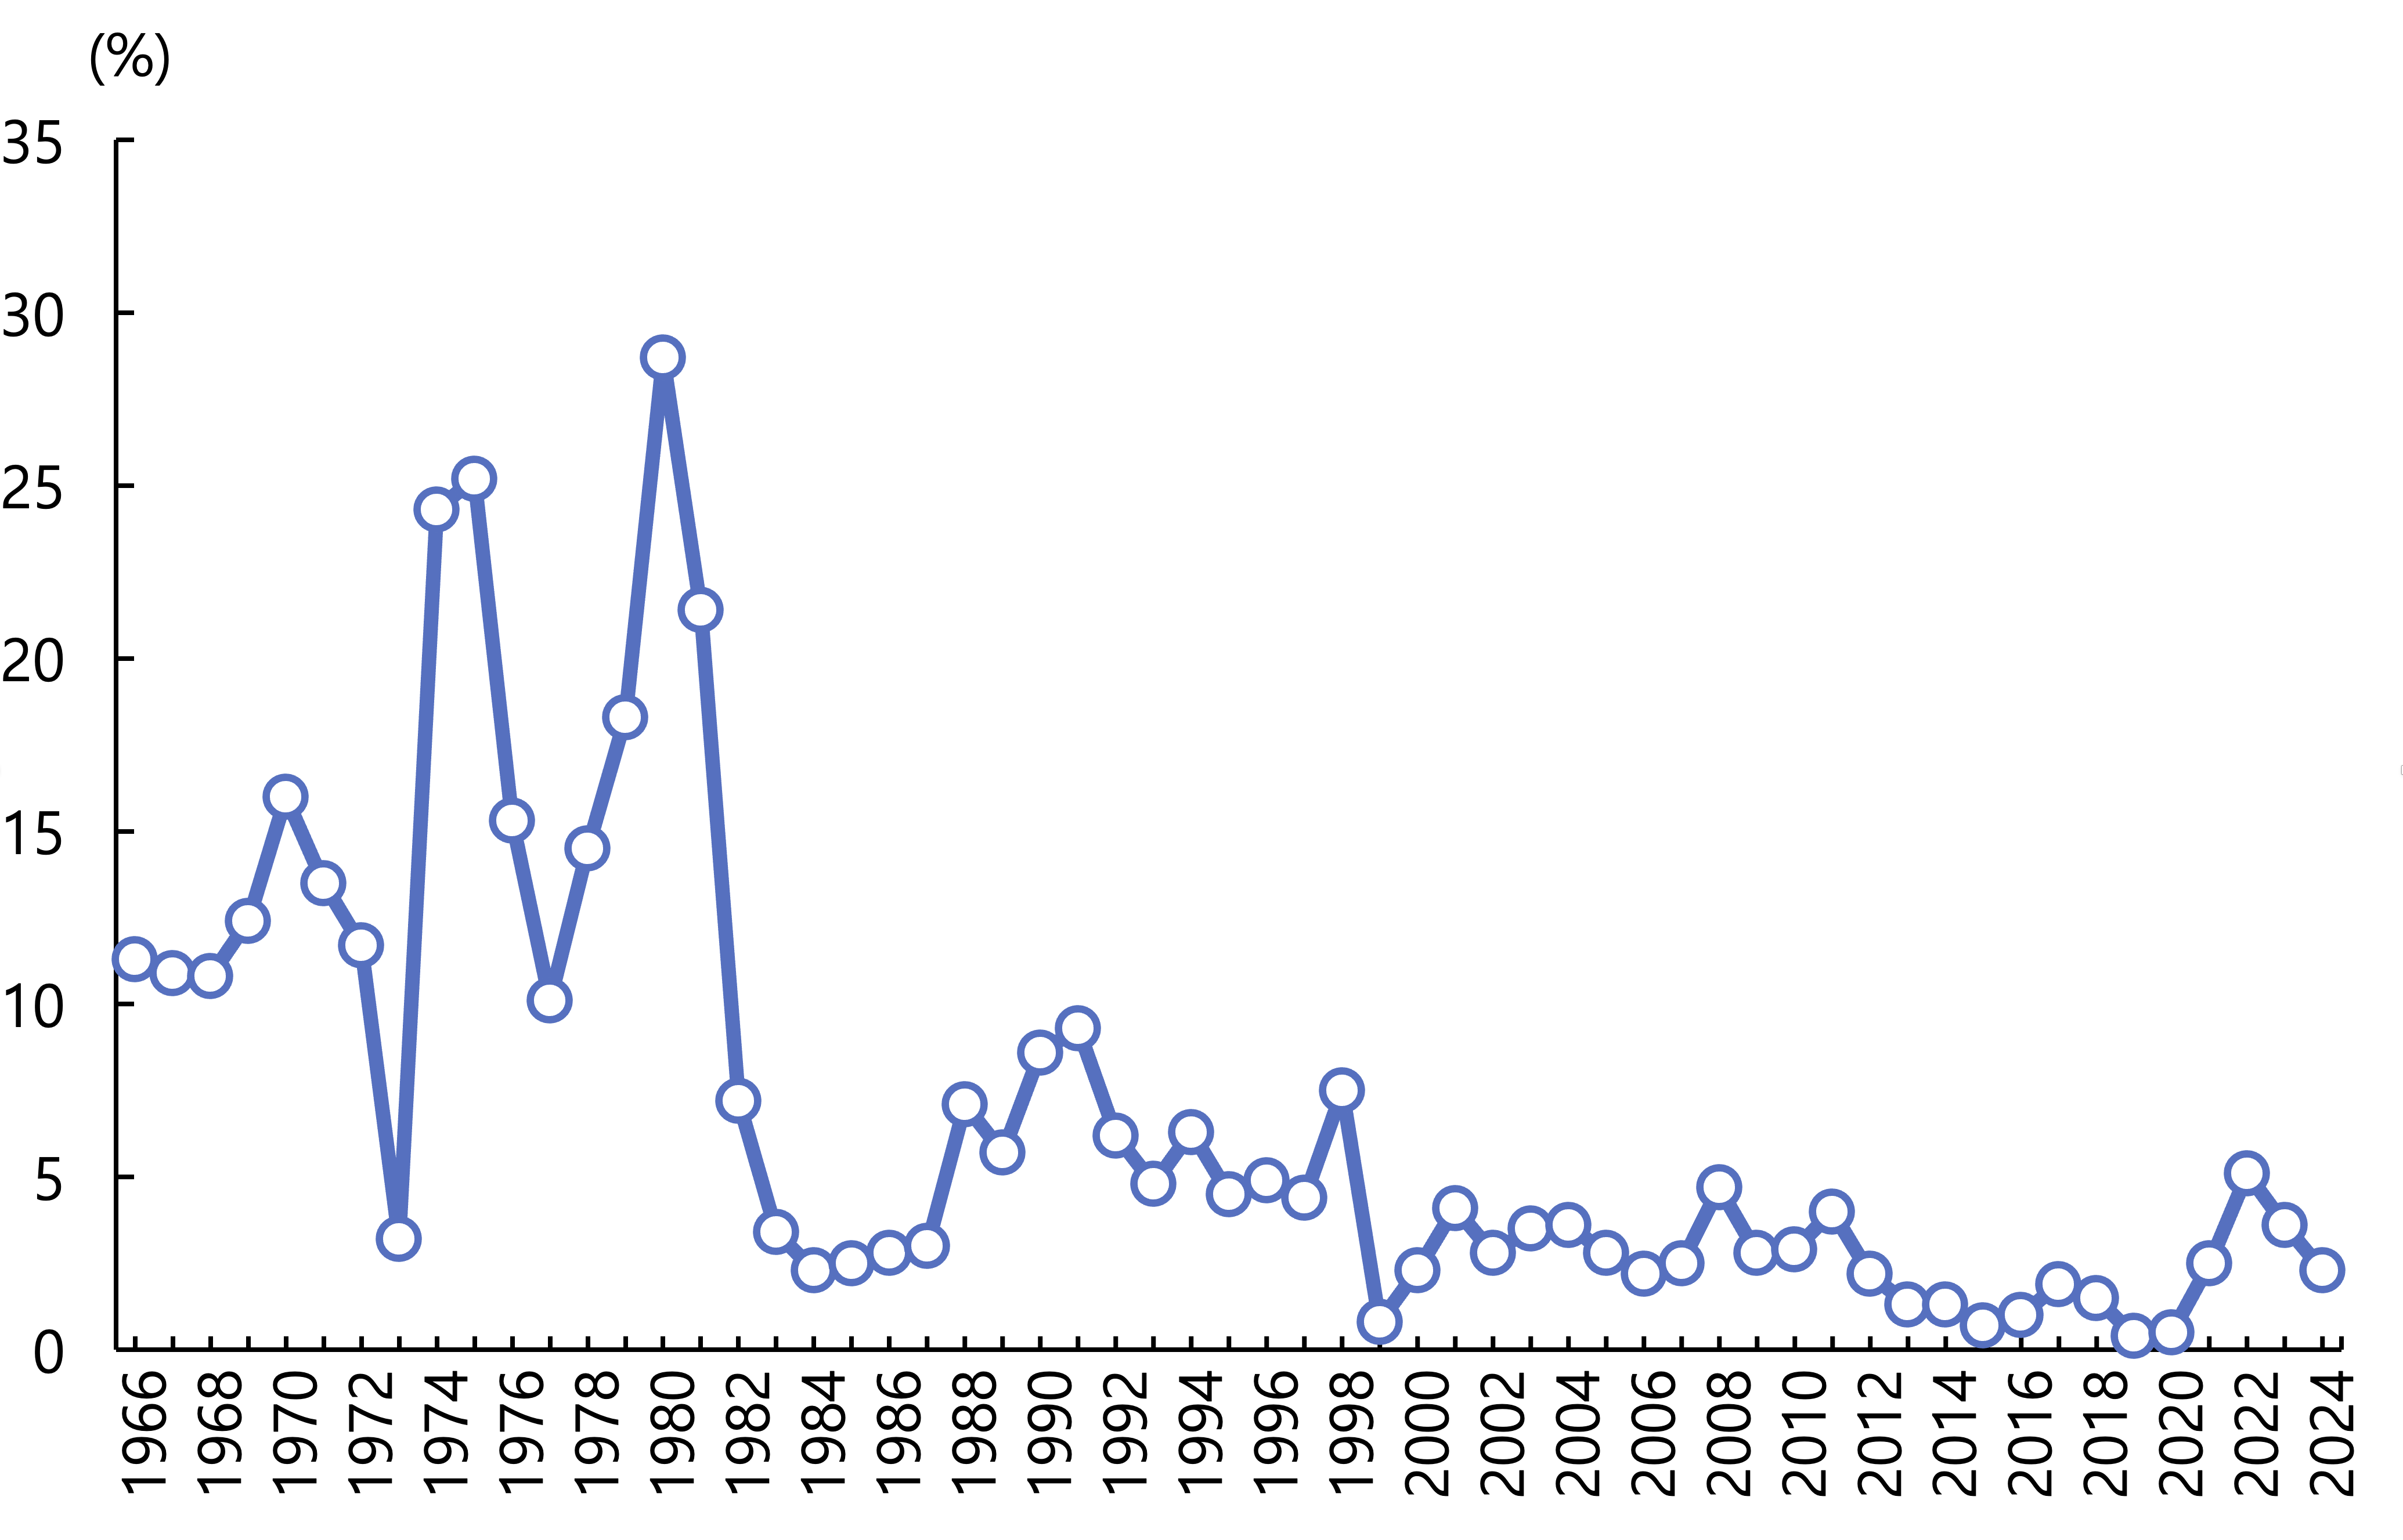
\includegraphics[width=.55\textwidth]{pic/fig_ineq_02.png}
    \end{figure}
    \begin{itemize}
        \item 효용을 극대화 하는 분배가 정당한 분배이다.
    \end{itemize}
\end{frame}

\begin{frame}[<+->]
\frametitle{소비수준}
    \begin{figure}
        \centering
        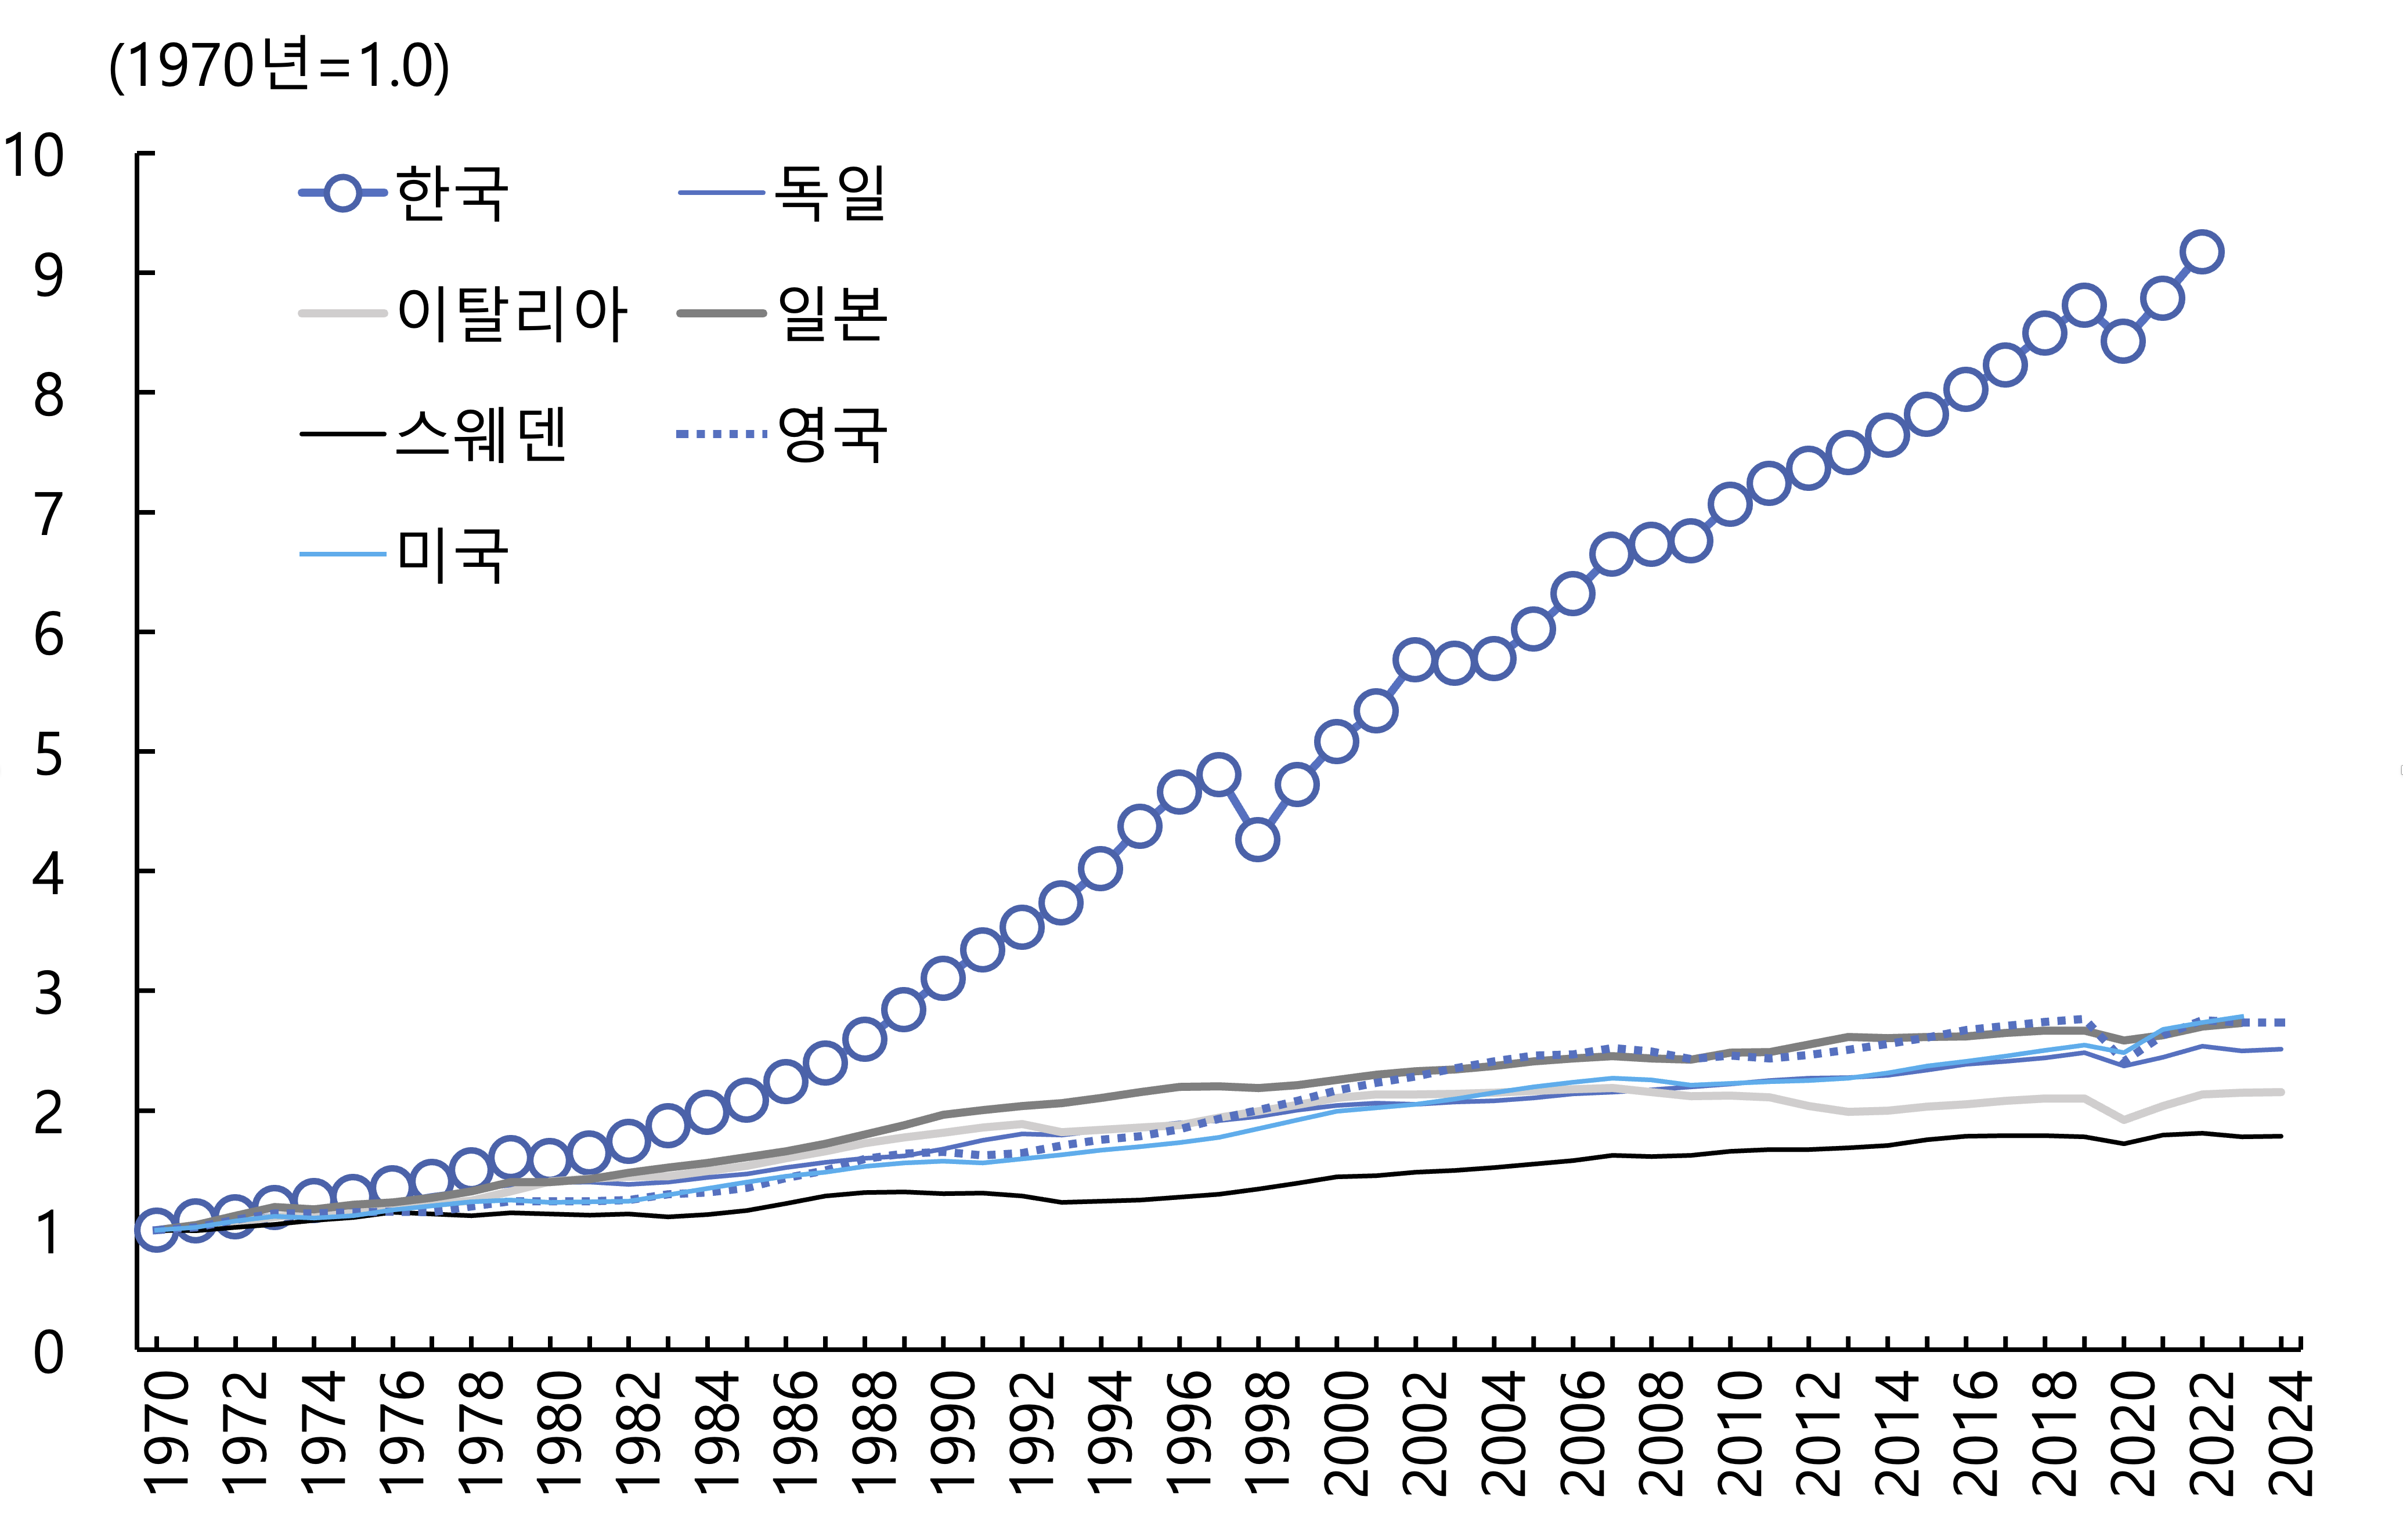
\includegraphics[width=.55\textwidth]{pic/fig_ineq_04.png}
    \end{figure}
    \begin{itemize}
        \item 효용을 극대화 하는 분배가 정당한 분배이다.
    \end{itemize}
\end{frame}

\subsection{분배}
\begin{frame}[<+->]
\frametitle{빈곤율}
    \begin{figure}
        \centering
        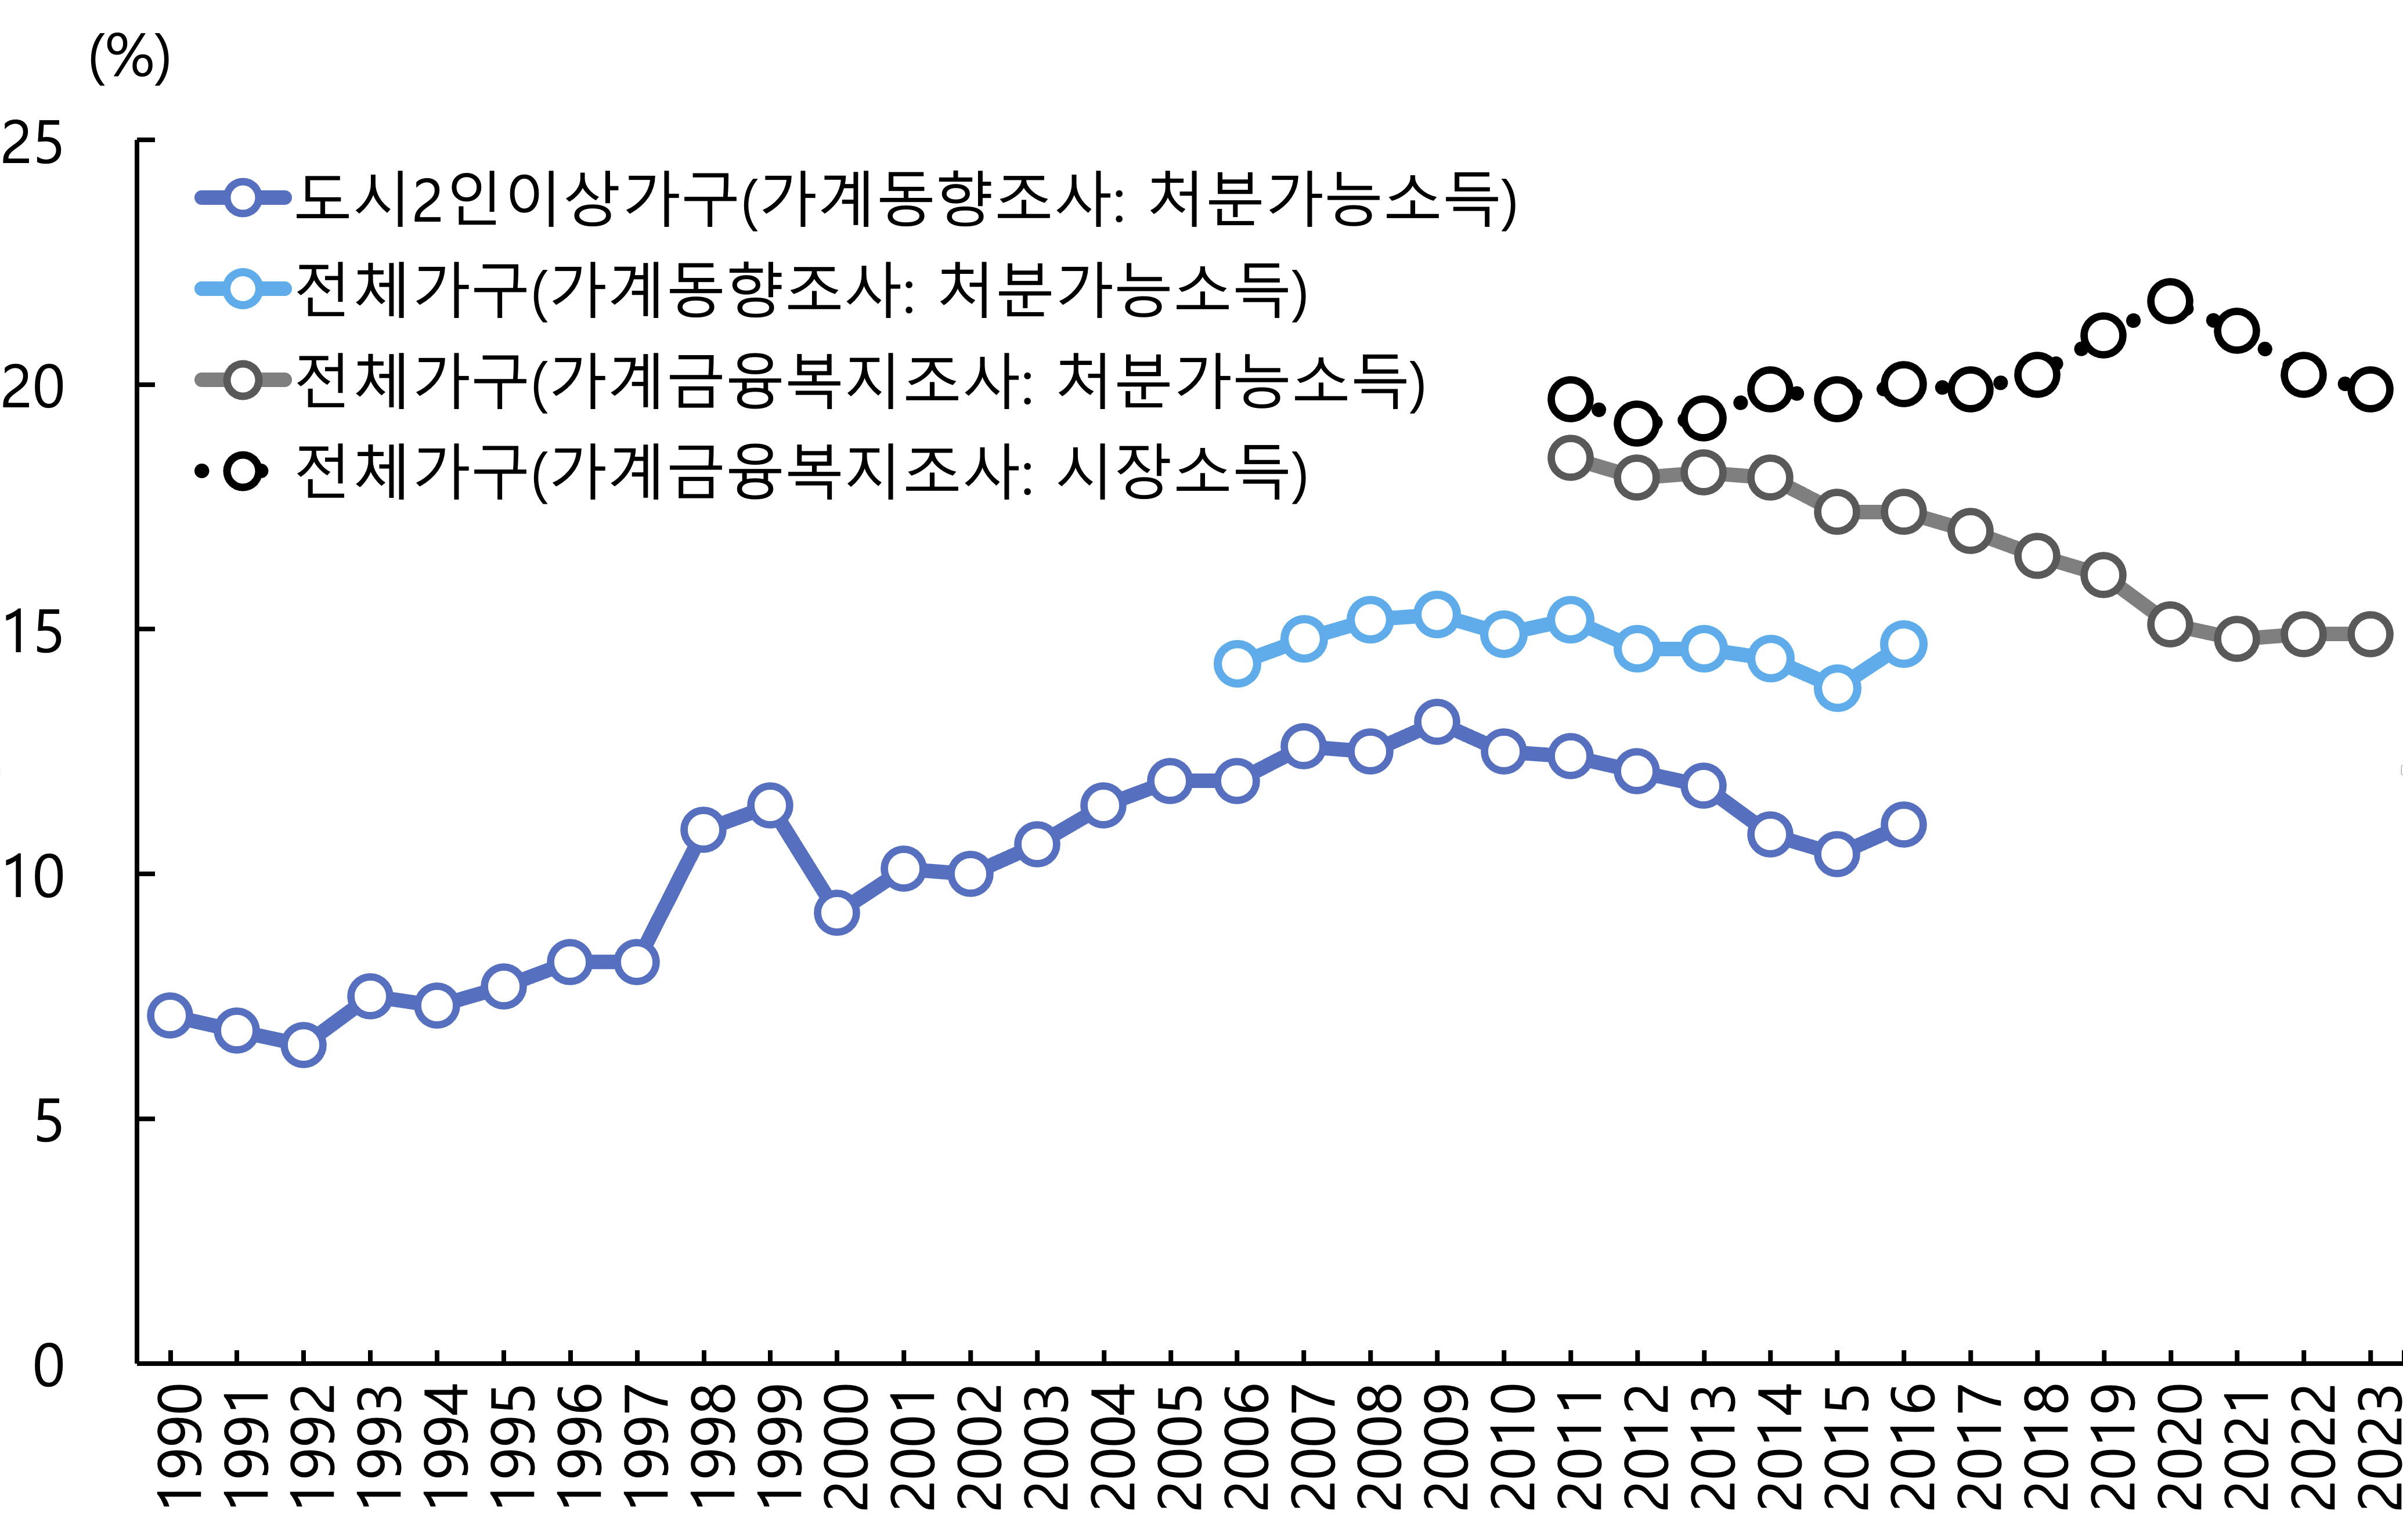
\includegraphics[width=.55\textwidth]{pic/fig_ineq_07.png}
    \end{figure}
    \begin{itemize}
        \item 효용을 극대화 하는 분배가 정당한 분배이다.
    \end{itemize}
\end{frame}

\begin{frame}[<+->]
\frametitle{지니계수}
    \begin{figure}
        \centering
        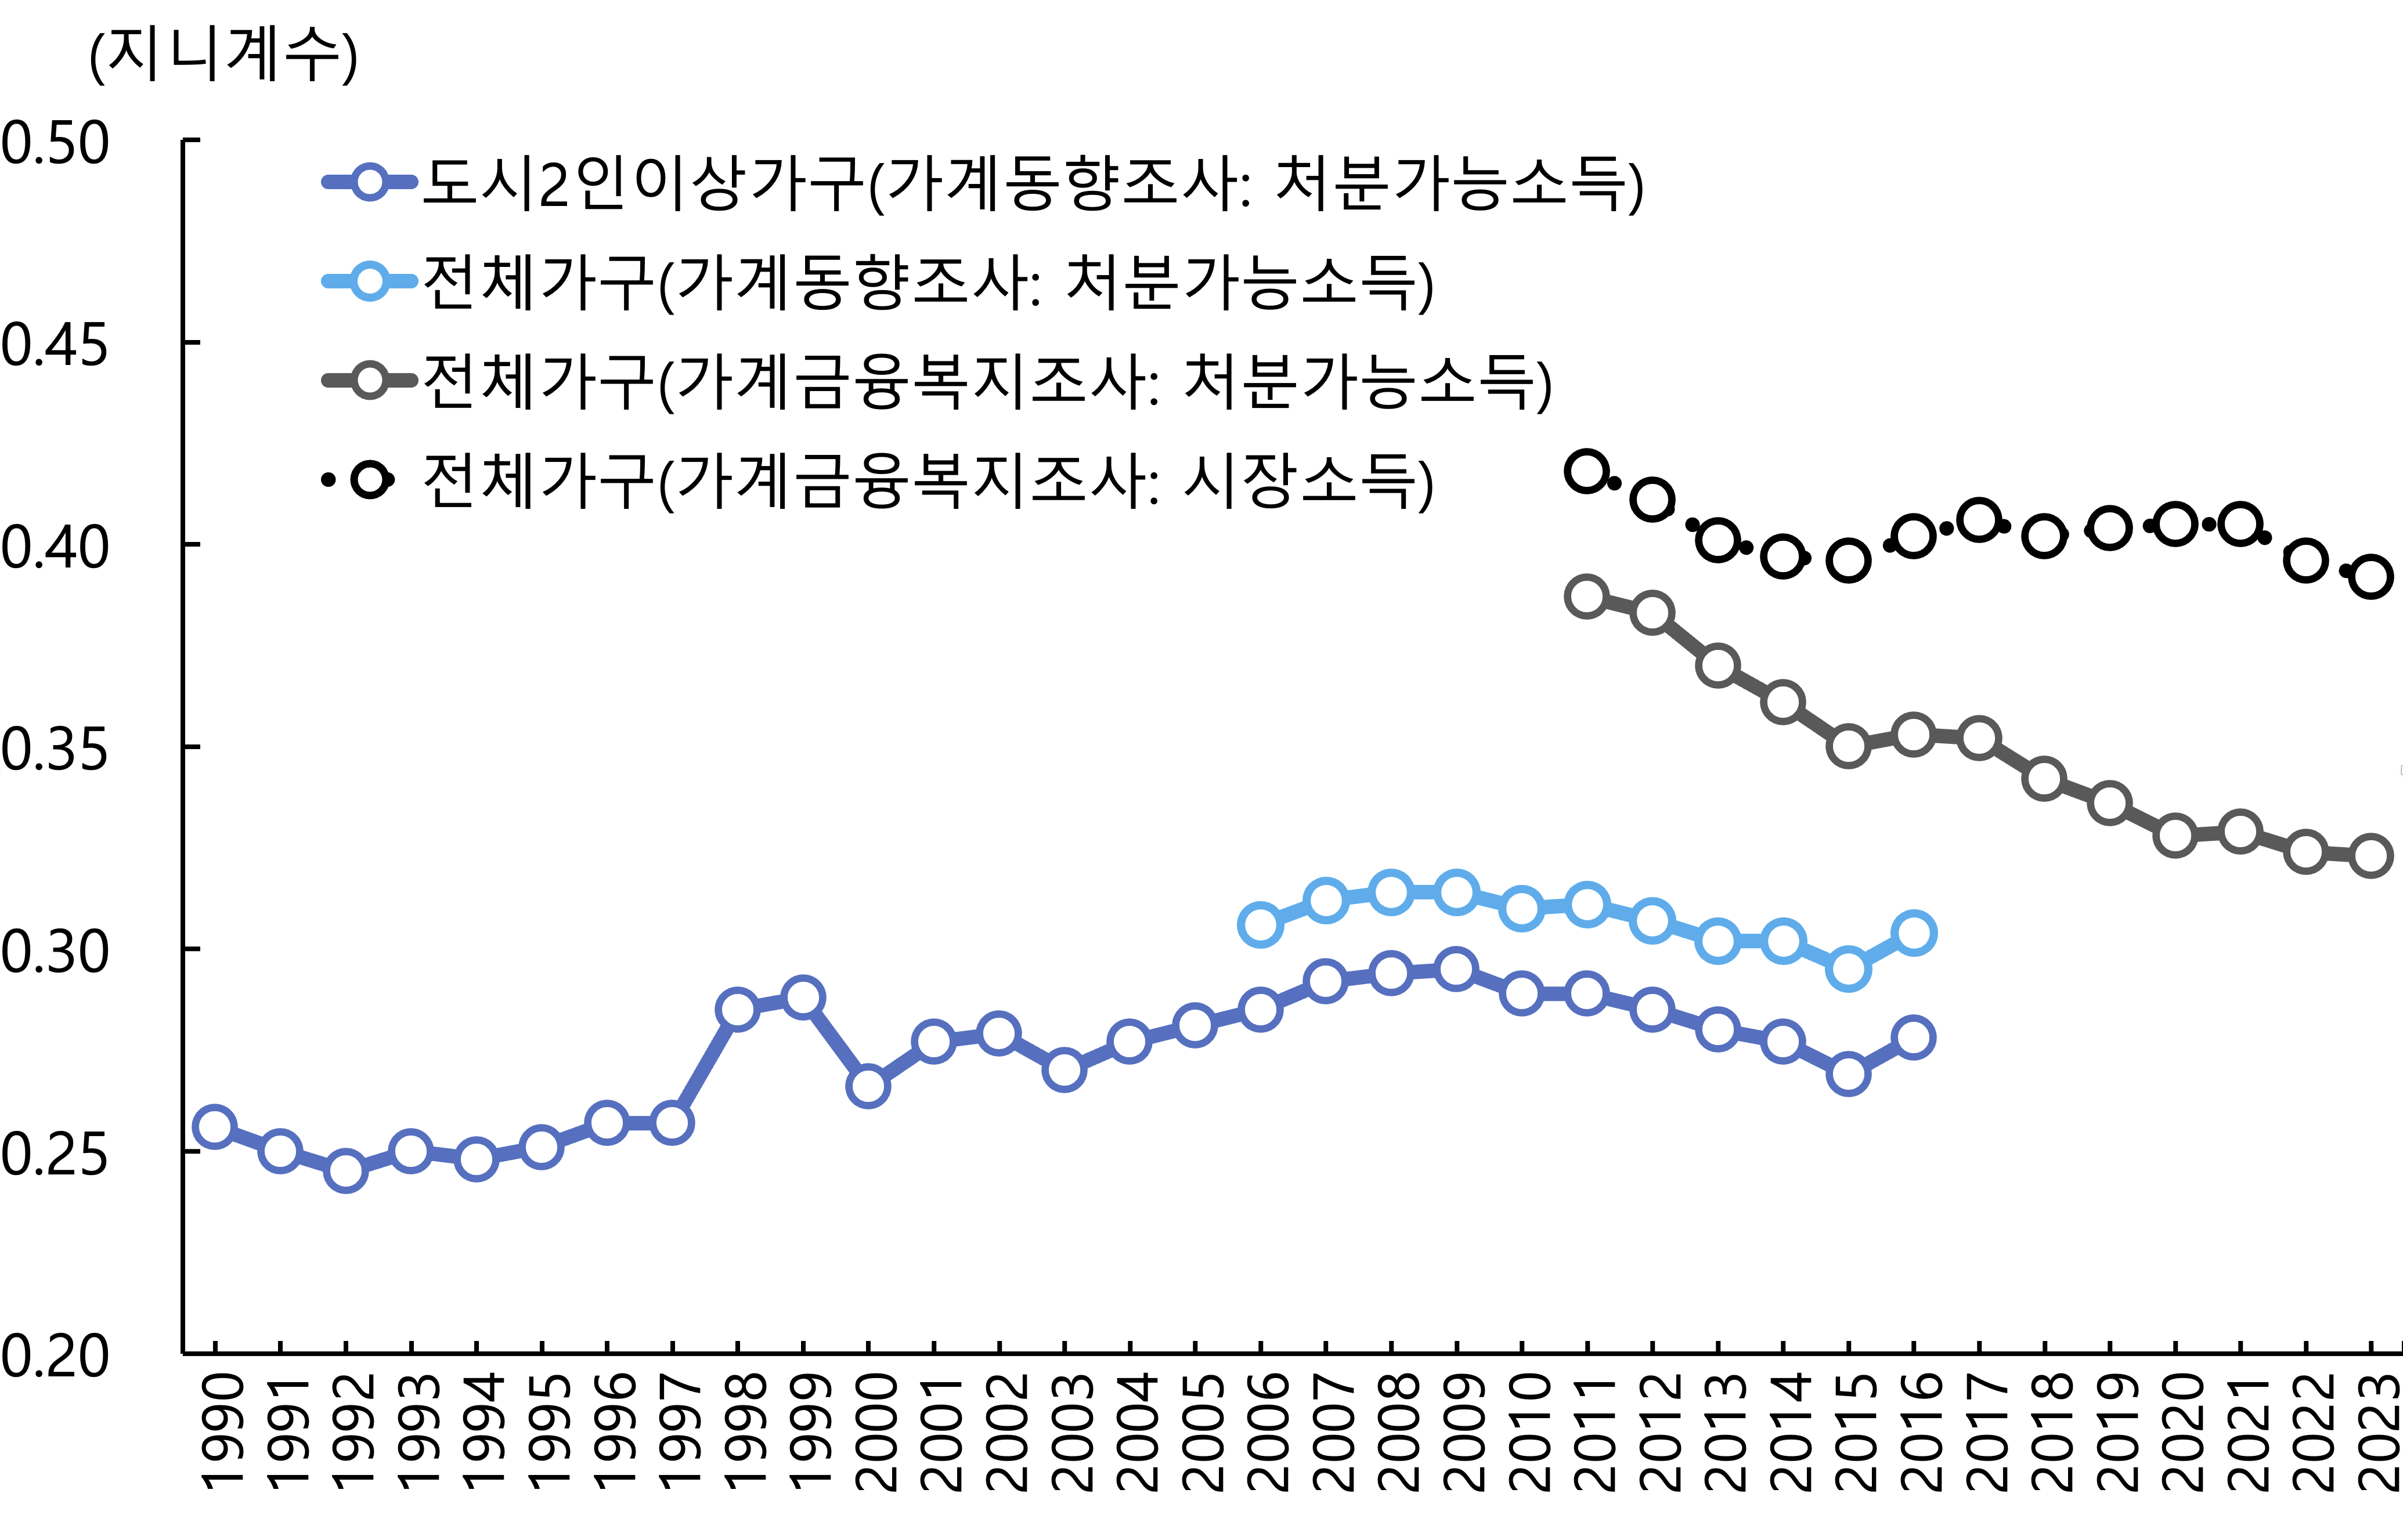
\includegraphics[width=.55\textwidth]{pic/fig_ineq_08.png}
    \end{figure}
    \begin{itemize}
        \item 효용을 극대화 하는 분배가 정당한 분배이다.
    \end{itemize}
\end{frame}

\begin{frame}[<+->]
\frametitle{소득 5분위 배율}
    \begin{figure}
        \centering
        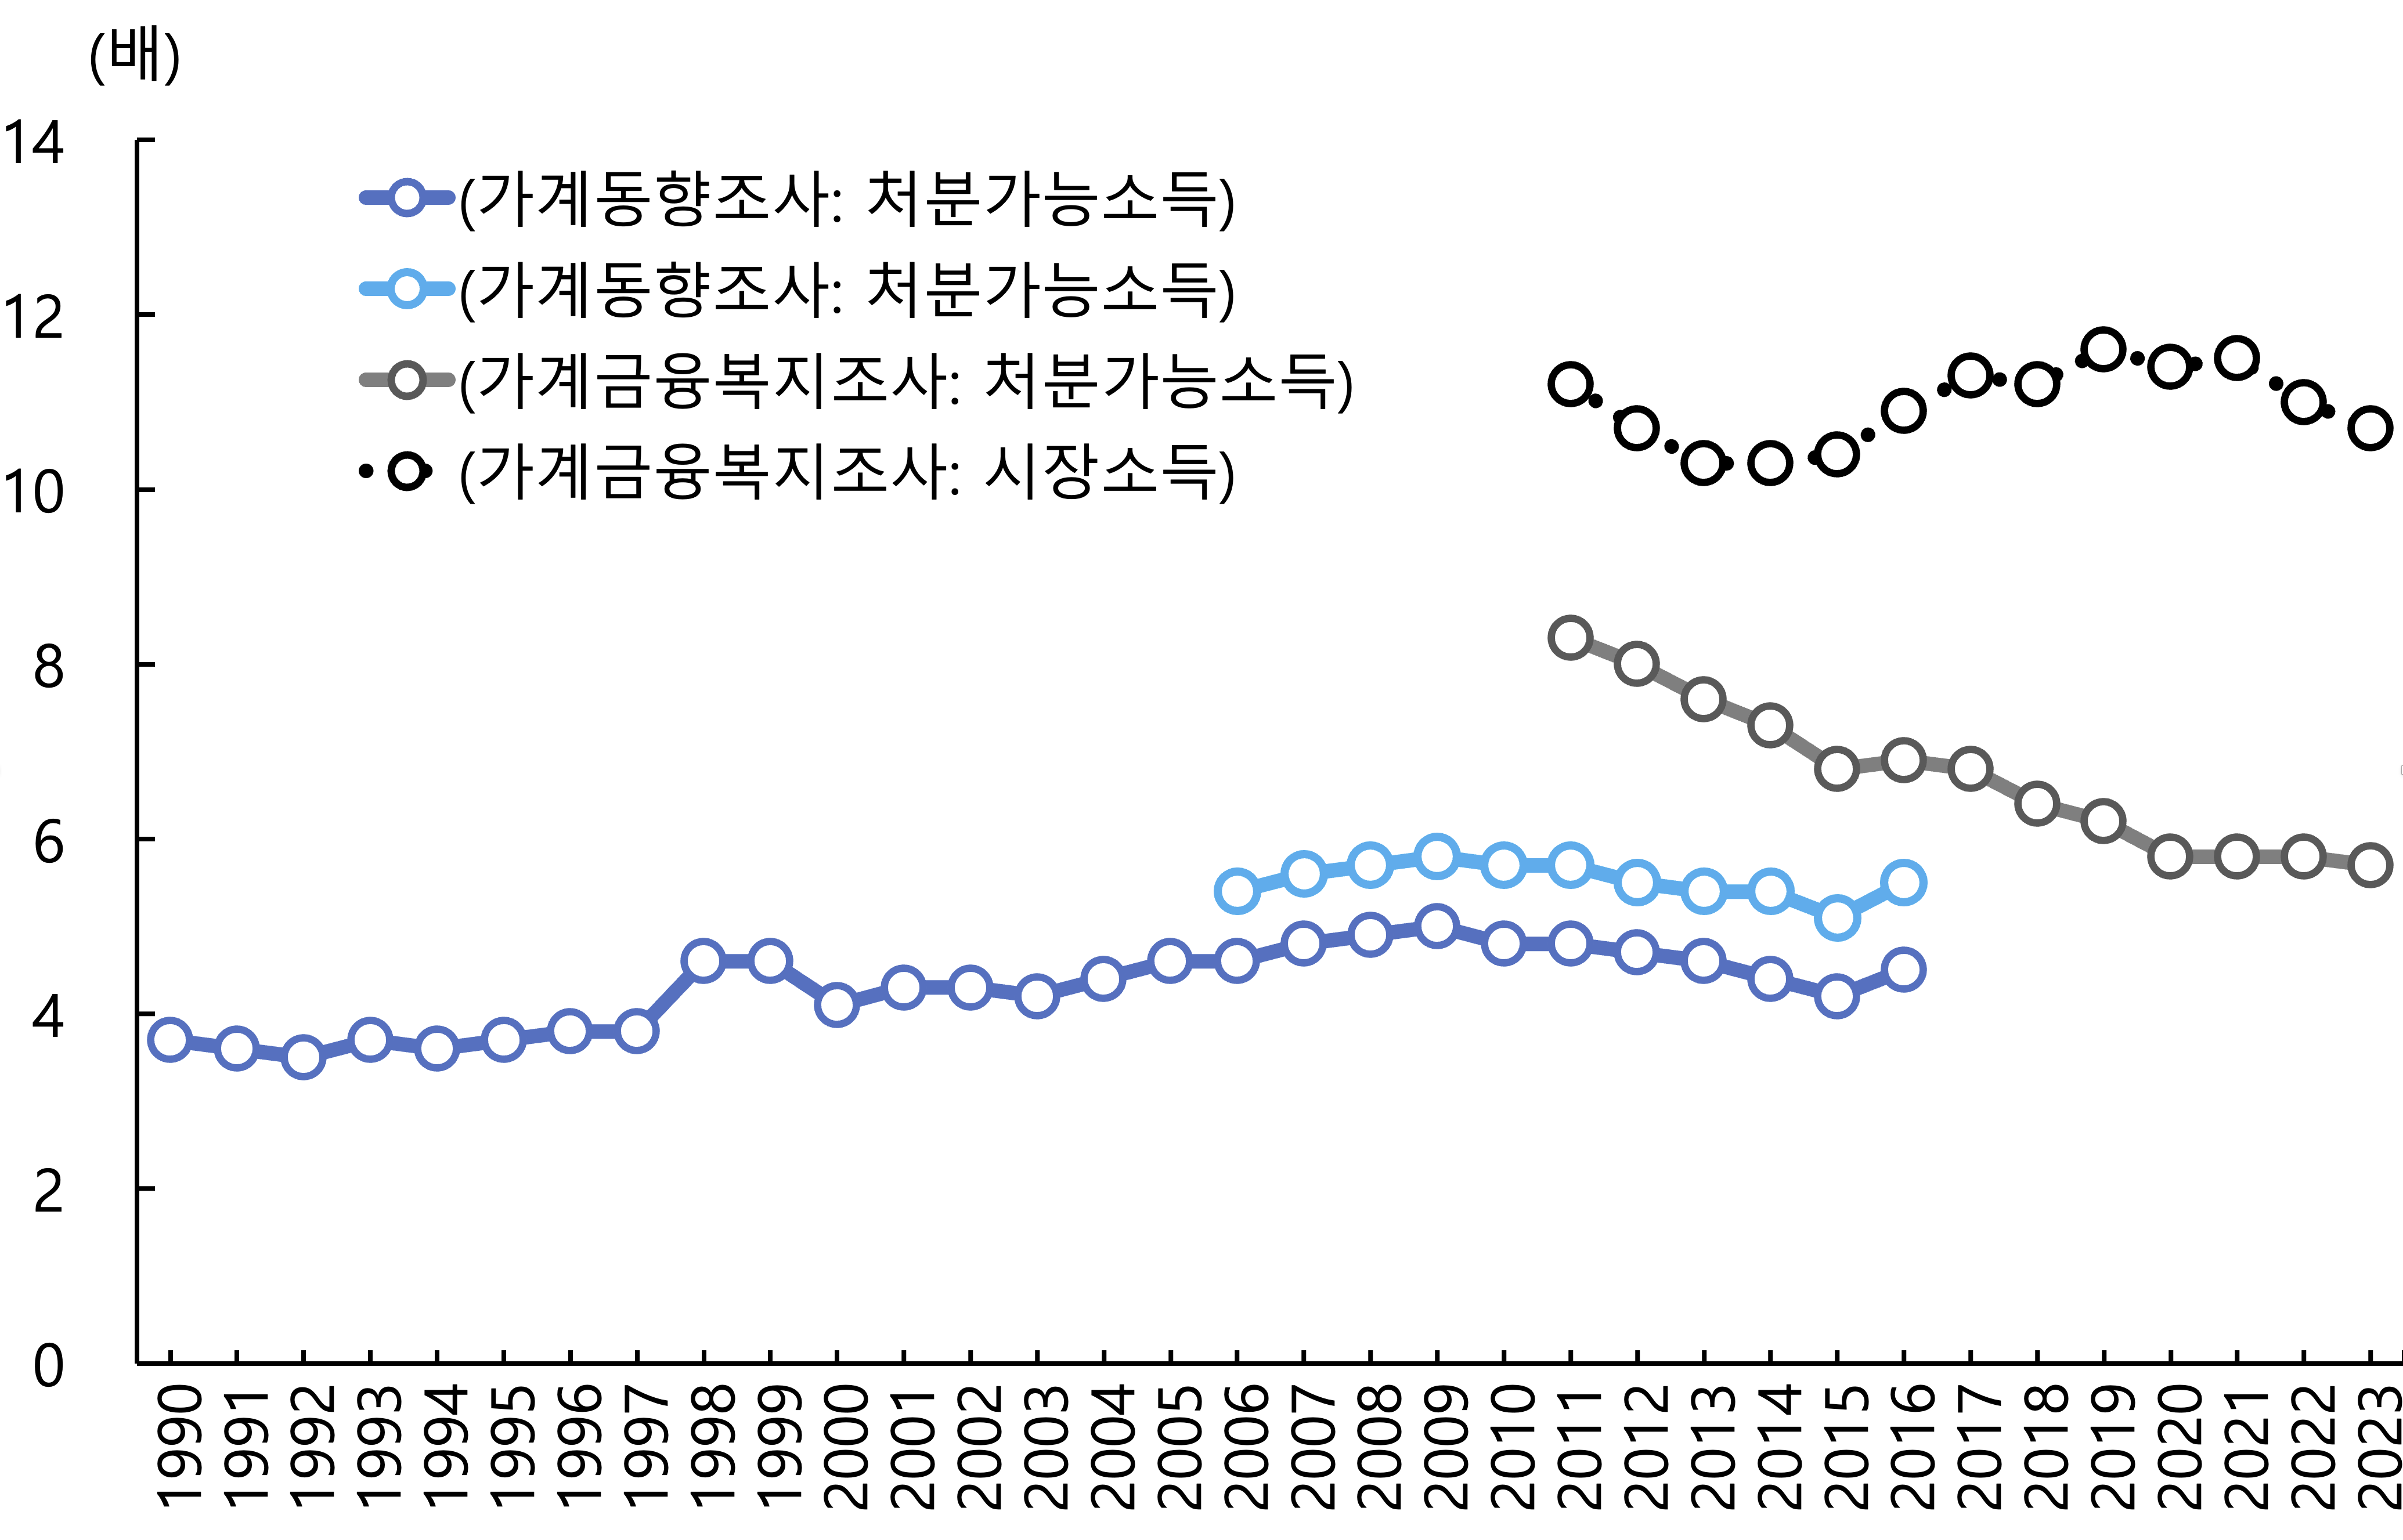
\includegraphics[width=.55\textwidth]{pic/fig_ineq_09.png}
    \end{figure}
    \begin{itemize}
        \item 효용을 극대화 하는 분배가 정당한 분배이다.
    \end{itemize}
\end{frame}

\begin{frame}[<+->]
\frametitle{주요국의 사회복지지출 추이}
    \begin{figure}
        \centering
        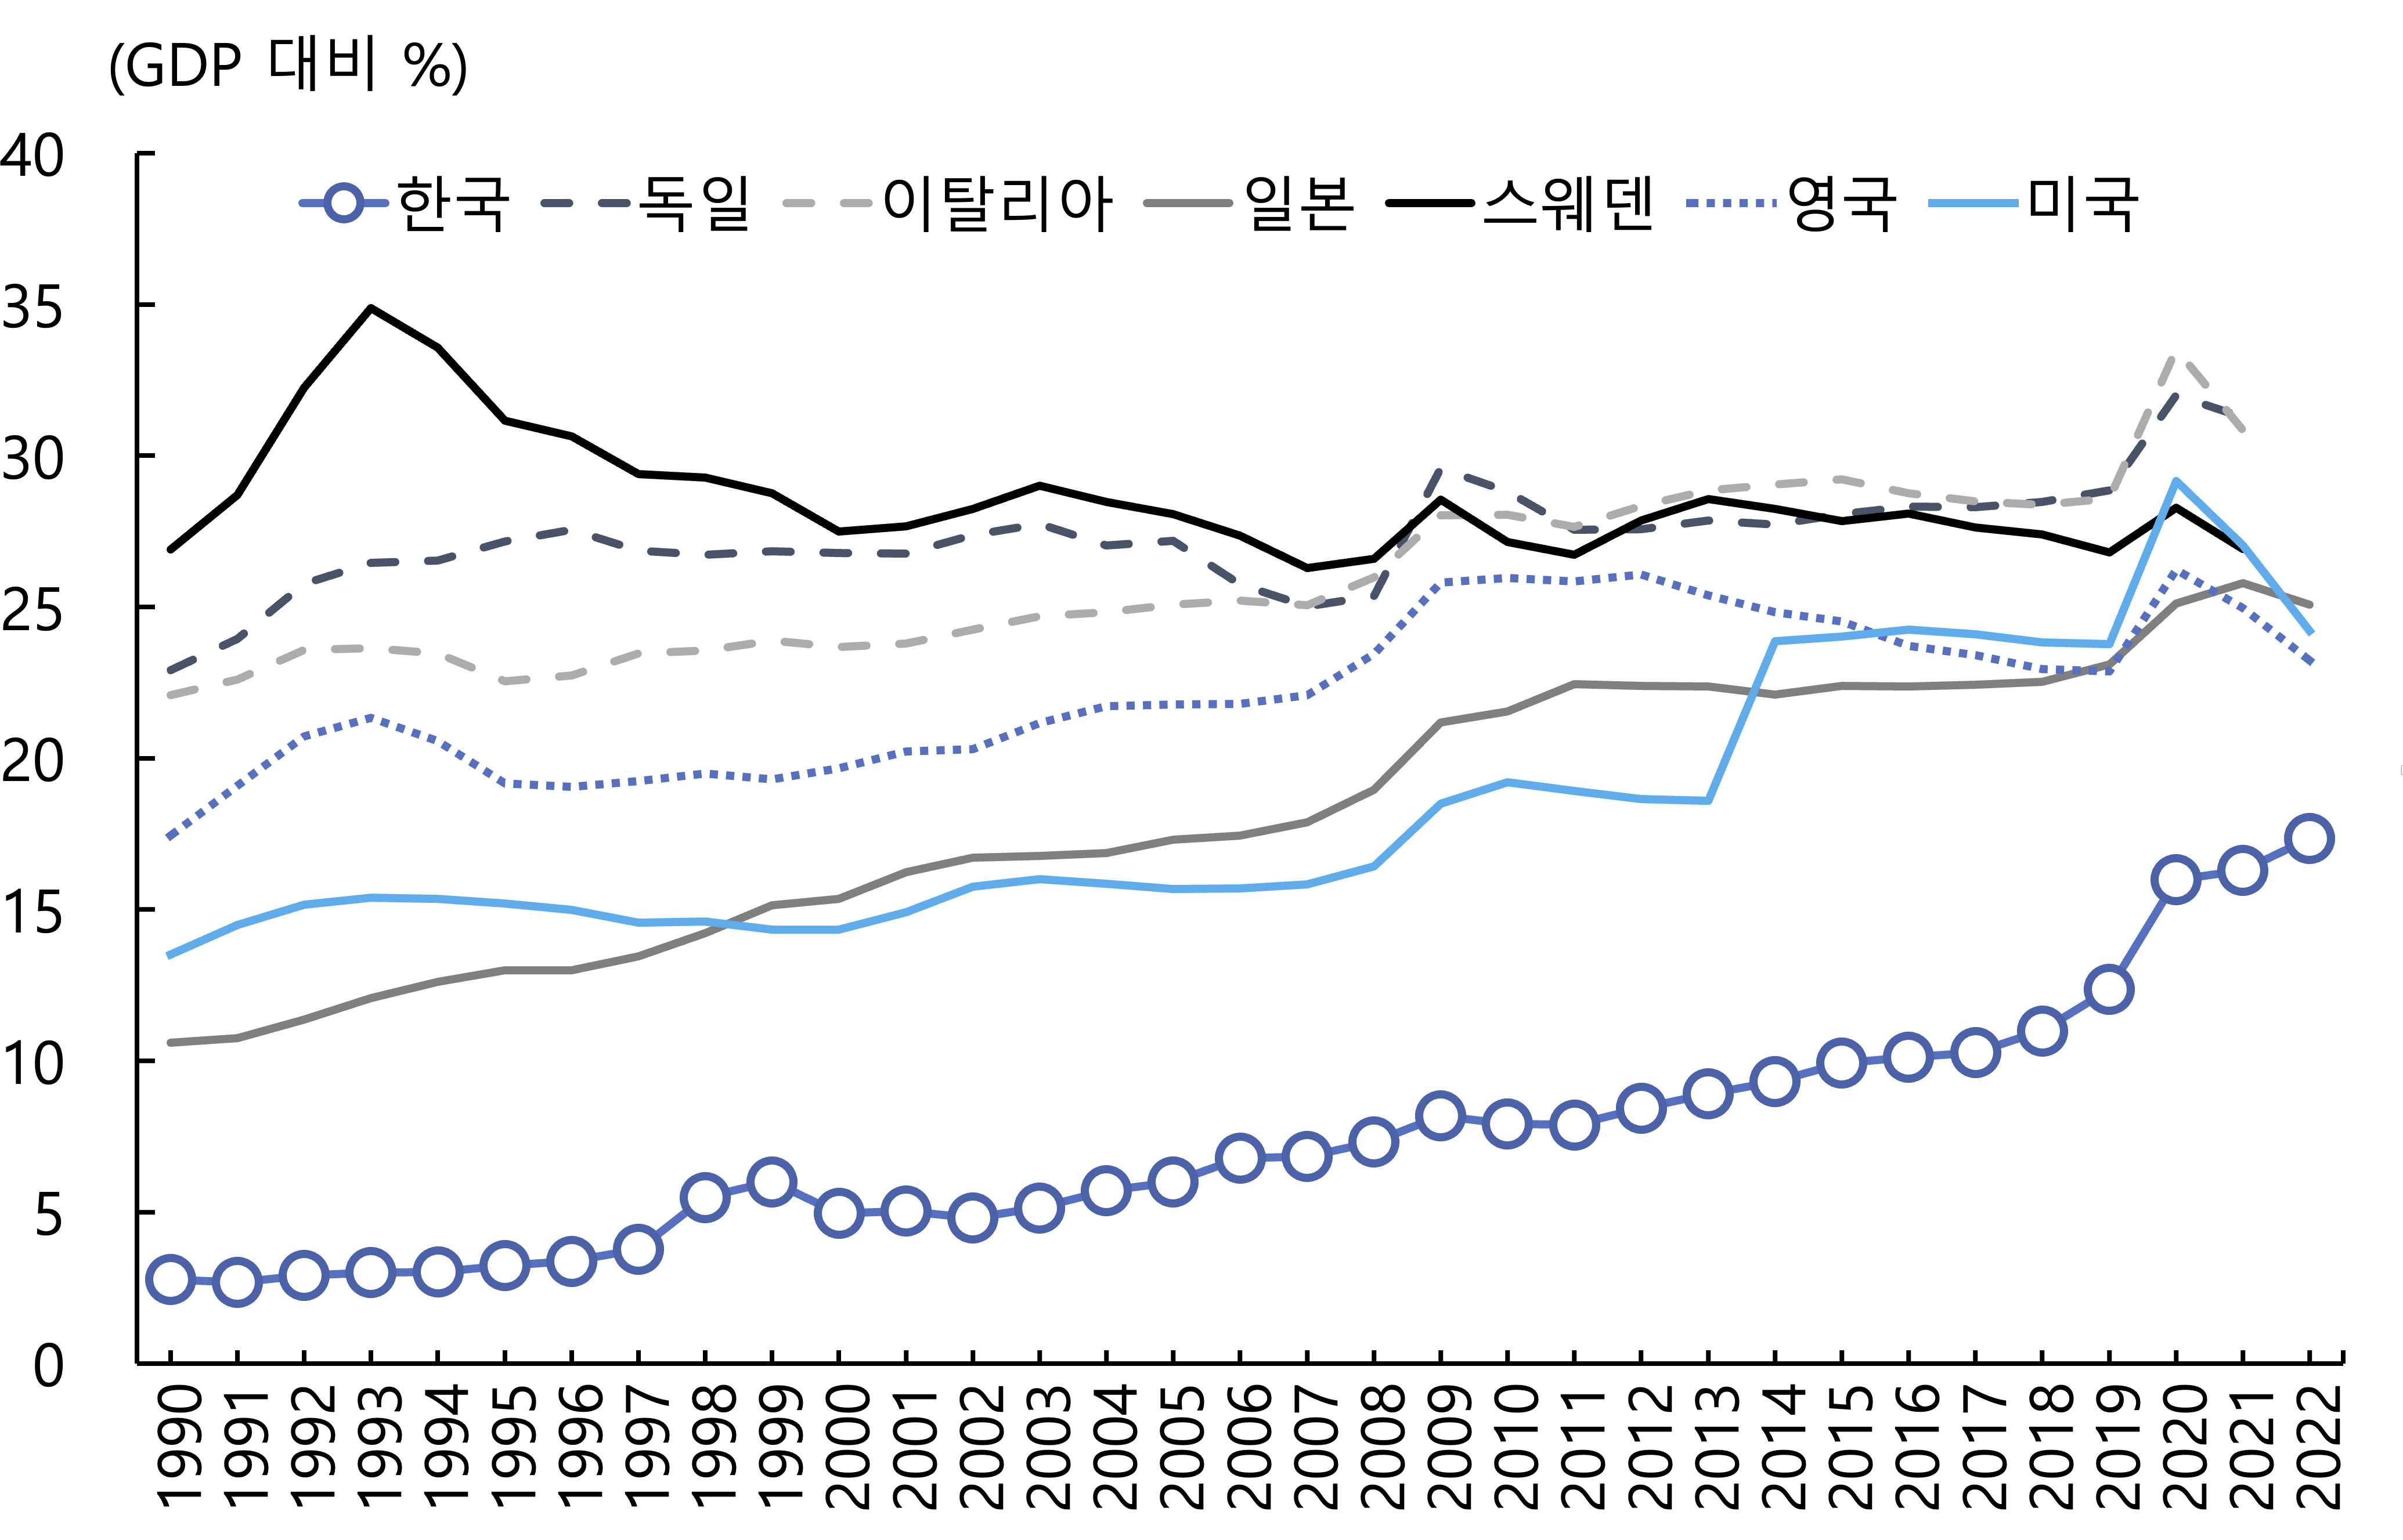
\includegraphics[width=.55\textwidth]{pic/fig_ineq_10.png}
    \end{figure}
    \begin{itemize}
        \item 효용을 극대화 하는 분배가 정당한 분배이다.
    \end{itemize}
\end{frame}

\begin{frame}[<+->]
\frametitle{가구유형별 소득에서 공적이전소득이 차지하는 비중}
    \begin{figure}
        \centering
        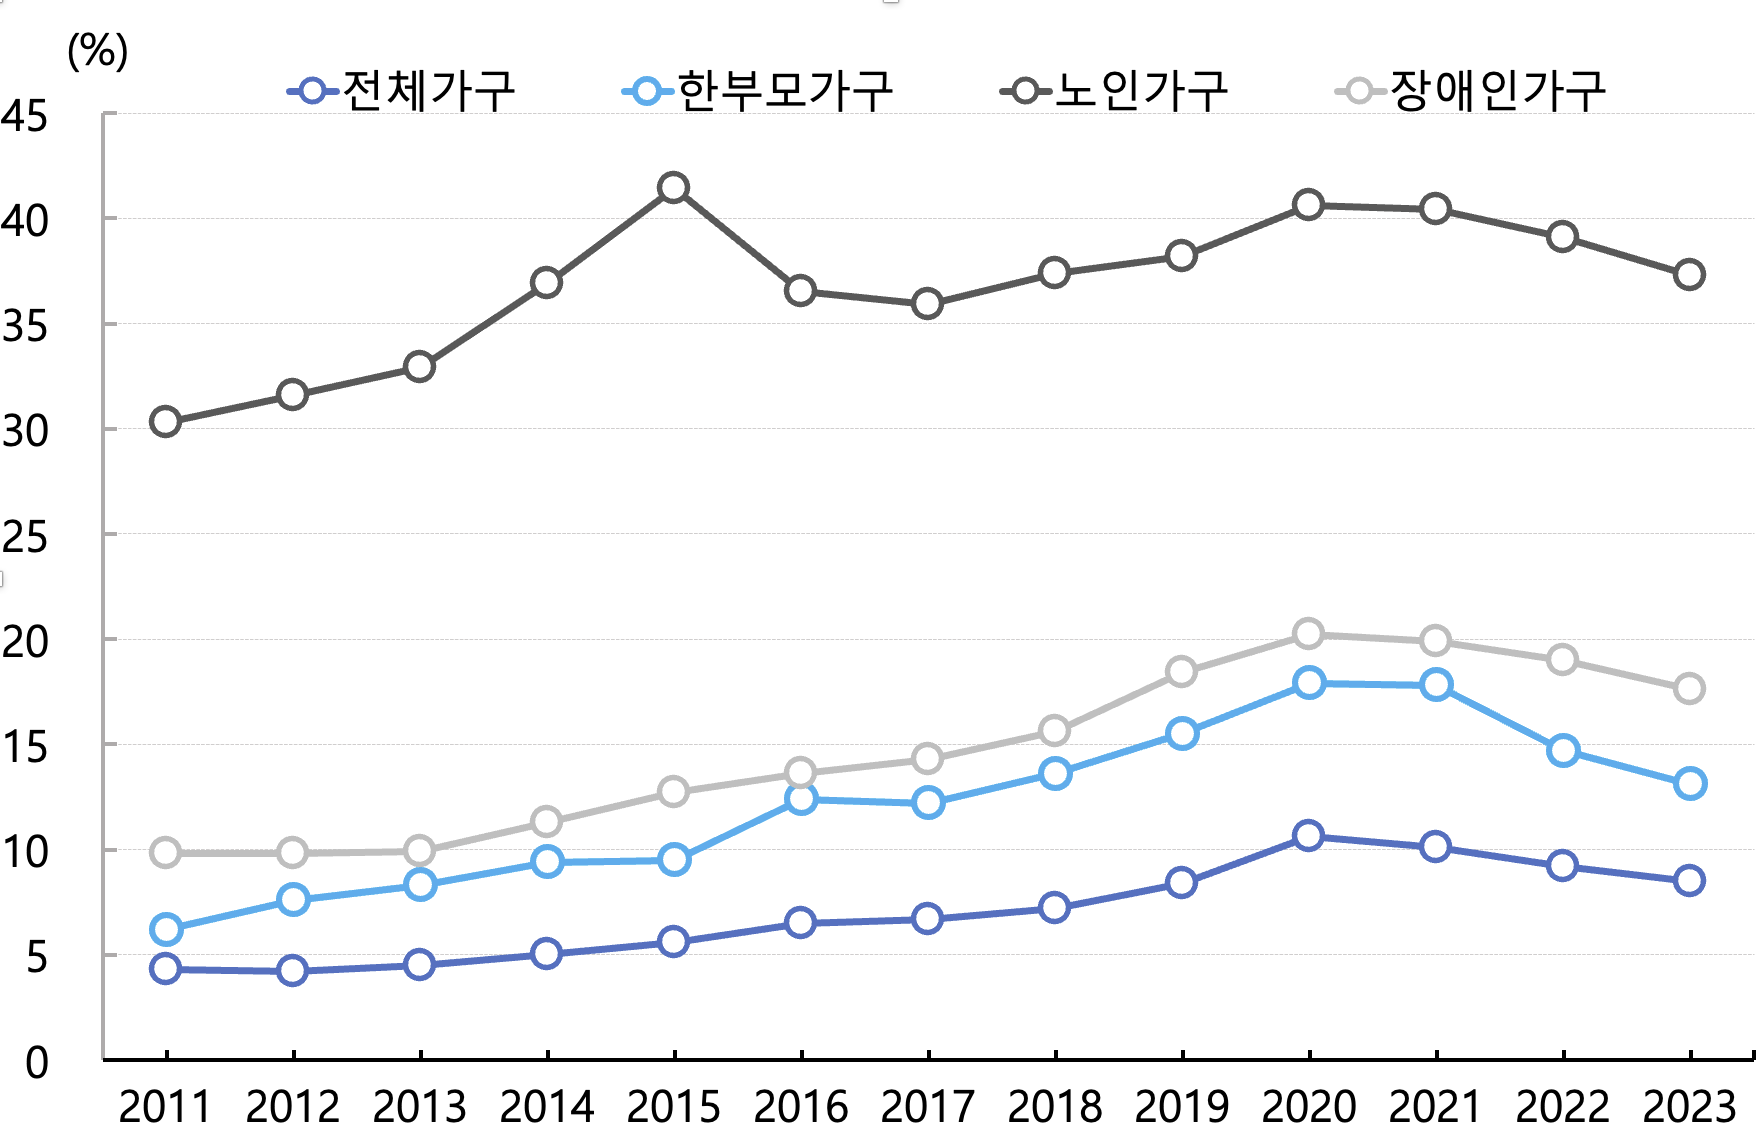
\includegraphics[width=.55\textwidth]{pic/fig_ineq_11.png}
    \end{figure}
    \begin{itemize}
        \item 효용을 극대화 하는 분배가 정당한 분배이다.
    \end{itemize}
\end{frame}
%------------------------------------------------
\end{document}
%------------------------------------------------
